\documentclass[pdflatex,sn-nature]{sn-jnl}
\usepackage{amsmath}
\usepackage{amssymb}
\usepackage[scaled=0.92]{helvet}
\usepackage{amsthm}
\newtheorem{proposition}{Proposition}
\newtheorem{corollary}{Corollary}
\usepackage{booktabs}
\usepackage{siunitx}
\sisetup{detect-weight=true,detect-family=true,mode=text}
\usepackage{xcolor}
\usepackage{tcolorbox}
\usepackage{tikz}
\usetikzlibrary{arrows.meta,positioning,calc,shapes.geometric,fit,backgrounds,decorations.pathreplacing}
% ---- Nature-style figure palette and styles ----
\definecolor{npblue}{HTML}{2E6CA4}
\definecolor{nporange}{HTML}{E08214}
\definecolor{npgreen}{HTML}{3F9B6E}
\definecolor{npred}{HTML}{C0392B}
\definecolor{nppurple}{HTML}{7B5EA7}
\definecolor{npslate}{HTML}{3A4A5A}
\tikzset{
  proc/.style={rounded corners=2pt,draw=npblue!55,fill=npblue!8,line width=0.6pt,align=center,inner sep=3.5pt,font=\small},
  data/.style={rounded corners=2pt,draw=black!35,fill=black!4,line width=0.6pt,align=center,inner sep=3.5pt,font=\small},
  good/.style={rounded corners=2pt,draw=npgreen!65,fill=npgreen!12,line width=0.6pt,align=center,inner sep=3pt,font=\small},
  bad/.style={rounded corners=2pt,draw=npred!65,fill=npred!10,line width=0.6pt,align=center,inner sep=3pt,font=\small},
  acc/.style={rounded corners=2pt,draw=nporange!70,fill=nporange!12,line width=0.6pt,align=center,inner sep=3pt,font=\small},
  flow/.style={-{Latex[length=2.0mm,width=1.6mm]},line width=0.7pt,draw=black!60},
  plab/.style={font=\bfseries\large},
  card/.style={draw=black!22,line width=0.6pt,fill=white,rounded corners=2pt},
  ax/.style={->,line width=0.5pt,draw=black!50,>=stealth},
}
\usepackage{algorithm}
\usepackage{algpseudocode}

% Red-flag helper for author-supplied items still to be filled (visible in the PDF).
\newcommand{\redflag}[1]{\textcolor{red}{[#1]}}

\raggedbottom

\begin{document}

\title[MatPCR]{Physics Is the Label: A Label-Free Benchmark and Verifier for the Physical Consistency of Materials Reasoning in Vision--Language and Language Models}

\author*[1]{\fnm{Hasan} \sur{Kurban}}\email{hkurban@hbku.edu.qa}
\author[1]{\fnm{Rasul} \sur{Khanbayov}}\email{rkhanbayov@hbku.edu.qa}
\author*[2]{\fnm{Mustafa} \sur{Kurban}}\email{mkurbanphys@gmail.com}

\affil*[1]{\orgdiv{College of Science and Engineering}, \orgname{Hamad Bin Khalifa University}, \orgaddress{\city{Doha}, \country{Qatar}}}
\affil[2]{\orgname{Ankara University}, \orgaddress{\city{Ankara}, \country{Turkey}}}

\abstract{Vision--language and language models increasingly interpret materials data, yet recent
benchmarks report that they frequently hallucinate invalid properties and violate
physical law. Evaluation has centered on matching a final answer to a scarce human label,
while discovery agents instead verify final proposals or the correctness of density
functional theory (DFT) execution. Neither measures the physical consistency of a model's
reasoning chain. We observe that materials data carries its own physics, which makes a
large class of materials reasoning verifiable without annotation. We introduce MatPCR, a
DFT-grounded, label-free benchmark whose programmatic oracles check diffraction geometry
through Bragg's law, scale bars, spectral peaks, and DFT-grounded stability, metallicity,
and property magnitude. We define the Physical-Consistency Rate (PCR) over image
and structure inputs; introduce Constraint-Grounded Self-Verification (a label-free
agentic loop) and show, against unaided self-refinement and generic re-prompting controls,
that its gain is attributable to the oracle signal rather than extra inference-time compute;
release an open verifier, useful in distribution but not transferring to any of six
held-out constraint types; and bound the reported PCR's error by an exact bias
term and a sampling term.}

\keywords{materials informatics, vision--language models, scientific reasoning, label-free evaluation, density functional theory}

\maketitle

\noindent\begin{tcolorbox}[colback=gray!6,colframe=gray!50,boxrule=0.5pt]
\textbf{Key contributions.} (1) We reframe materials-model evaluation from answer accuracy to the physical
consistency of the reasoning chain, checkable without human labels for a large,
well-defined class of physical errors, across vision--language and language inputs. (2) We release MatPCR: programmatic,
modality-specific physical oracles including DFT-grounded property checks. (3) We
define PCR, a metric with bootstrap confidence intervals and a paired significance
test, and prove an exact bias identity relating measured to true PCR and, under
independent sampling, a high-probability bound on the reported estimate's total error.
(4) We fine-tune and release an open physical-consistency verifier, a useful
in-distribution detector that does not transfer to any of six held-out constraint types,
and benchmark it against zero-shot LLM-judge and self-confidence baselines. (5) We
propose CGSV, a label-free agentic self-verification loop, isolate its effect from
unaided self-refinement and equal-compute re-prompting controls, and give a protocol to measure
its effect on violations.
\end{tcolorbox}

\section*{Introduction}
% =====================================================================
Materials data is governed by physics that is, in large part, programmatically
checkable. A micrograph's scale bar fixes its spatial calibration; a powder
diffraction pattern's peak positions follow from a crystal structure and the source
through Bragg's law; a crystal's thermodynamic stability is set by its energy
relative to a convex hull; and a computed property has a definite sign and order of
magnitude. Vision--language models (VLMs) and language models (LLMs) are now
routinely asked to reason over such data, and a large literature evaluates them on
materials tasks;\cite{lai2025materials,npj2026vlmeval,choudhary2025microscopygpt,li2024mmsci}
classical computer-vision pipelines for microstructure and defect analysis predate
them.\cite{holm2020cv,li2018defect}

The problem this creates is now well documented. Materials benchmarks report that
general-purpose models hallucinate invalid property values\cite{llm4matbench2024,lai2025materials}
and benchmark their spatial and structural reasoning over crystals,\cite{atomworld2025}
motivating purpose-built multimodal materials models.\cite{matterchat2026} Beyond
materials, recent work shows vision--language models violate basic physical law,
for example failing conservation under transformation;\cite{conservationbench2026}
in response, open vision--language models now add physics-grounded reinforcement
learning and inference-time self-verification to strengthen physics-problem
reasoning.\cite{p1vl2026} Across domains, a shared response has emerged:
a model's reasoning should be audited against laws or logic in a
reference-free way, whether through conservation-grounded metrics or deterministic
formal checks.\cite{conservationbench2026,neurosymclinical2026}

That literature, like multimodal evaluation generally, scores the final answer
against human labels. A parallel and fast-growing line builds discovery agents that
couple language models with simulation and first-principles tools to propose and
screen candidates;\cite{dreams2025,crystalyse2025,mapps2025,atomagents2024,llmatdesign2024,matpc2025,kang2024chatmof,zhang2024honeycomb,survey2025aimat}
some verify the physics of final proposals, for example through physics-aware
rejection sampling,\cite{physrej2025} mitigate hallucination during DFT
execution,\cite{dreams2025} or pre-screen candidates with machine-learned
interatomic potentials before DFT.\cite{genbaselines2025,chgnet2023} General-domain
methods verify chains of thought via visual grounding or generic
programs,\cite{corgi2025,mmverify2025,vlmr3_2026,prove2024} but against visual
evidence or generic programs rather than domain physics, and on general benchmarks
rather than materials. A third line builds verifiers and process-reward models that
score reasoning steps;\cite{processbench2025,compassverifier2025,t1verify2025} these
have driven reinforcement learning from verifiable rewards in mathematics and code,
where correctness is programmatically checkable,\cite{deepseekr1_2025} but
verification has remained under-specified for scientific reasoning, where answers are
free-form and references are scarce.\cite{scirlvr2026} Across all three lines, the
physical consistency of the model's reasoning chain on materials data is neither
measured nor made reusable. Yet that is what
determines whether a model can be trusted inside an analysis or screening pipeline:
a chain that reads a 100~nm scale bar and then reports a 10~$\mu$m feature, assigns
a peak to a $2\theta$ the stated phase cannot produce, or calls a structure stable
that lies far above the convex hull, is wrong on its face. Checking the chain against
external physics is also less susceptible than outcome- or judge-based verification to a
plausible but physically inadmissible chain: a model's stated reasoning need not
faithfully reflect its computation, so an unfaithful trace can satisfy a final-answer or
judge check while resting on physics that does not hold, whereas a programmatic oracle
tests the admissibility of the stated claims directly.\cite{faithflow2026}

We make one observation: materials data contains its own
ground truth for a large class of reasoning errors, and with first-principles access
that ground truth extends from geometry to computed physics. These constraints are
checkable with no human annotation, yielding a label-free signal that scales with the
available public data and that applies equally to image inputs (VLMs) and
structure or text inputs (LLMs). This brings to materials the reference-free correctness
signal that has driven progress in mathematics and code, though here the oracles are
imperfect-precision necessary conditions rather than the effectively exact checkers of
those domains. We turn this into MatPCR, a benchmark and a set of
oracles including DFT-grounded property checks; the Physical-Consistency Rate (PCR);
Constraint-Grounded Self-Verification (CGSV); and an open, fine-tuned verifier
released as a reusable artifact (Fig.~\ref{fig:teaser}).

The distinction from each neighboring line is precise. Against materials benchmarks
that score answers or property predictions,\cite{lai2025materials,llm4matbench2024,atomworld2025,matterchat2026}
we score the physical consistency of the reasoning chain rather than the final
answer, with a label-free oracle. Against physical-law evaluations of model
reasoning,\cite{conservationbench2026,p1vl2026} we ground the check in materials
characterization and first-principles DFT, span both image and structure inputs, and
release a verifier and a label-free self-verification loop rather than only a diagnostic.
Against discovery agents,\cite{dreams2025,physrej2025} we measure reasoning-chain
consistency and act on oracle-flagged violations, rather than screen final proposals or
run DFT. Against general verifiers
and process-reward models,\cite{processbench2025,compassverifier2025,t1verify2025}
including recent step-level verifiers for scientific or structured reasoning,\cite{sciprm2026,vprm2026}
we supply a domain-specific, physics- and DFT-grounded, label-free signal for a setting
where verification was previously under-specified. Those verifiers need an answer key, a
tool call, or gold reasoning annotation; our oracle needs none of these. The two closest contemporaneous
efforts use physics as a programmatic signal for materials models but stop short of the
reasoning chain: one benchmarks vision--language models on X-ray-diffraction peak
indexing, grading the final indexed answer against structure-derived labels on the
diffraction modality alone,\cite{crystalxrdbench2026} and the other uses DFT-computed
energies and band gaps as a label-free reward, but as a binary exact-match signal on the
final answer during reinforcement-learning training rather than a chain-level
consistency measure at evaluation and inference time.\cite{matpref2026} MatPCR differs
from both in scoring the physical consistency of the intermediate chain, spanning four
oracle modalities, and closing a label-free self-verification loop with a released
verifier. No single prior effort provides a label-free, reasoning-chain-level,
multi-oracle, materials-specific consistency benchmark with a self-verification loop and
a released verifier.

This work also extends a line of research by the present authors on multimodal
resources and benchmarks for crystalline
materials,\cite{polat2025crysmtm,polat2025rcrystals} on machine-learning property
prediction for nanomaterials,\cite{polat2025quantumshellnet,polat2024multimodalnp} on
benchmarking model hallucination,\cite{abdaljalil2025halluverse} and on
physics-grounded benchmarks for dynamic systems.\cite{khanbayov2026iris} MatPCR is
distinct from each: rather than providing a dataset, scoring generation or property
prediction, or measuring text factuality, it measures the physical consistency of the
reasoning chain itself and acts on the violations it finds, with label-free, DFT-grounded
oracles.

% Figure 1: teaser
\begin{figure}[t]
\centering
\resizebox{\linewidth}{!}{%
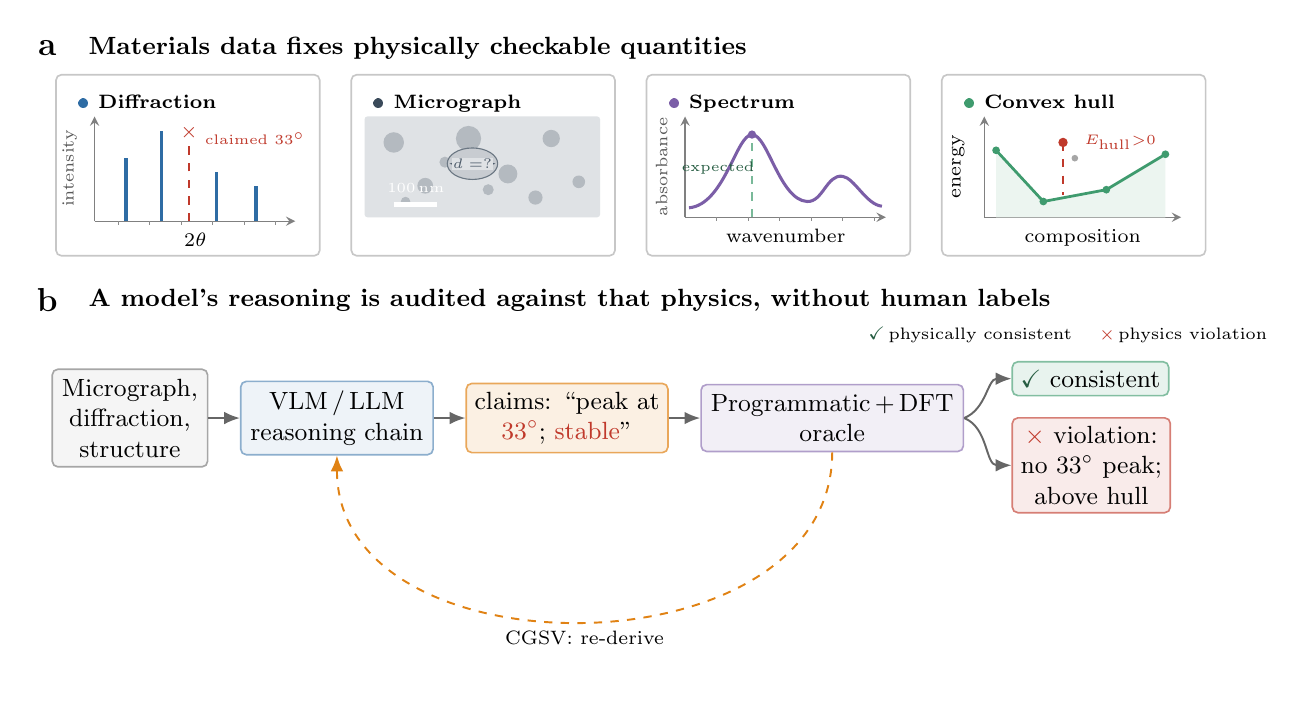
\begin{tikzpicture}[font=\sffamily]
\node[plab] at (-0.1,5.25){a};
\node[font=\small\bfseries,anchor=west] at (0.3,5.25){Materials data fixes physically checkable quantities};

% ---- card i: diffraction ----
\begin{scope}[shift={(0,2.6)}]
  \node[card,minimum width=3.35cm,minimum height=2.3cm,anchor=south west] at (0,0){};
  \node[font=\scriptsize\bfseries,anchor=north west] at (0.16,2.18){\textcolor{npblue}{\textbullet}\ Diffraction};
  \draw[ax] (0.5,0.45)--(3.05,0.45);
  \draw[ax] (0.5,0.45)--(0.5,1.78);
  \foreach \x in {0.8,1.2,1.6,2.0,2.4,2.8}\draw[black!45,line width=0.4pt](\x,0.45)--(\x,0.40);
  \foreach \x/\h in {0.9/0.80,1.35/1.15,2.05/0.62,2.55/0.45}
    \draw[npblue,line width=1.2pt] (\x,0.45)--(\x,{0.45+\h});
  % claimed-but-forbidden peak
  \draw[npred,line width=0.8pt,dashed] (1.7,0.45)--(1.7,1.45);
  \node[npred,font=\scriptsize] at (1.7,1.58){$\times$};
  \node[npred,font=\fontsize{5}{6}\selectfont,anchor=west] at (1.78,1.5){claimed $33^\circ$};
  \node[font=\scriptsize,anchor=north] at (1.78,0.42){$2\theta$};
  \node[font=\fontsize{6}{7}\selectfont,rotate=90,anchor=south,black!65] at (0.40,1.12){intensity};
\end{scope}

% ---- card ii: micrograph ----
\begin{scope}[shift={(3.75,2.6)}]
  \node[card,minimum width=3.35cm,minimum height=2.3cm,anchor=south west] at (0,0){};
  \fill[npslate!16,rounded corners=1pt] (0.18,0.5) rectangle (3.17,1.78);
  \foreach \x/\y/\r in {0.55/1.45/0.13, 0.95/0.9/0.10, 1.5/1.5/0.16, 2.0/1.05/0.12, 2.55/1.5/0.11, 2.9/0.95/0.08, 1.2/1.2/0.07, 2.35/0.75/0.09, 0.7/0.7/0.06, 1.75/0.85/0.07}
    \fill[npslate!38] (\x,\y) circle (\r);
  % feature to measure
  \draw[npslate!75,fill=npslate!28] (1.55,1.18) ellipse (0.32 and 0.2);
  \draw[{Latex[length=1.2mm]}-{Latex[length=1.2mm]},npslate!90,line width=0.5pt] (1.25,1.18)--(1.85,1.18);
  \node[font=\fontsize{5}{6}\selectfont,npslate!90,fill=npslate!16,inner sep=0.4pt] at (1.55,1.18){$d=?$};
  % scale bar
  \draw[white,line width=1.6pt] (0.55,0.66)--(1.1,0.66);
  \node[white,font=\fontsize{5.5}{6}\selectfont,anchor=south] at (0.83,0.69){100\,nm};
  \node[font=\scriptsize\bfseries,anchor=north west] at (0.16,2.18){\textcolor{npslate}{\textbullet}\ Micrograph};
\end{scope}

% ---- card iii: spectrum ----
\begin{scope}[shift={(7.5,2.6)}]
  \node[card,minimum width=3.35cm,minimum height=2.3cm,anchor=south west] at (0,0){};
  \draw[ax] (0.5,0.5)--(3.05,0.5);
  \draw[ax] (0.5,0.5)--(0.5,1.78);
  \foreach \x in {0.9,1.3,1.7,2.1,2.5,2.9}\draw[black!45,line width=0.4pt](\x,0.5)--(\x,0.45);
  \draw[nppurple,line width=1.1pt] (0.55,0.62) .. controls (1.0,0.66) and (1.15,1.55) .. (1.35,1.55)
     .. controls (1.55,1.55) and (1.7,0.72) .. (2.05,0.7)
     .. controls (2.25,0.69) and (2.3,1.05) .. (2.5,1.02)
     .. controls (2.65,1.0) and (2.8,0.66) .. (3.0,0.64);
  \fill[nppurple] (1.35,1.55) circle (1.5pt);
  \draw[npgreen!70,line width=0.8pt,dashed](1.35,0.5)--(1.35,1.5);
  \node[font=\fontsize{5}{6}\selectfont,npgreen!60!black,anchor=south] at (0.92,0.92){expected};
  \node[font=\scriptsize,anchor=north] at (1.78,0.47){wavenumber};
  \node[font=\fontsize{6}{7}\selectfont,rotate=90,anchor=south,black!65] at (0.40,1.14){absorbance};
  \node[font=\scriptsize\bfseries,anchor=north west] at (0.16,2.18){\textcolor{nppurple}{\textbullet}\ Spectrum};
\end{scope}

% ---- card iv: convex hull ----
\begin{scope}[shift={(11.25,2.6)}]
  \node[card,minimum width=3.35cm,minimum height=2.3cm,anchor=south west] at (0,0){};
  \draw[ax] (0.55,0.5)--(3.05,0.5);
  \draw[ax] (0.55,0.5)--(0.55,1.78);
  % stability region shading under hull
  \fill[npgreen!10] (0.7,1.35)--(1.3,0.7)--(2.1,0.85)--(2.85,1.3)--(2.85,0.5)--(0.7,0.5)--cycle;
  \draw[npgreen,line width=1.0pt] (0.7,1.35)--(1.3,0.7)--(2.1,0.85)--(2.85,1.3);
  \foreach \p in {(0.7,1.35),(1.3,0.7),(2.1,0.85),(2.85,1.3)}\fill[npgreen]\p circle (1.4pt);
  % off-hull gray points
  \fill[black!35] (1.7,1.25) circle (1.2pt);
  % red unstable point with drop line
  \fill[npred] (1.55,1.45) circle (1.7pt);
  \draw[npred,line width=0.6pt,dashed] (1.55,1.45)--(1.55,0.78);
  \node[npred,font=\fontsize{5}{6}\selectfont,anchor=west] at (1.7,1.45){$E_{\mathrm{hull}}{>}0$};
  \node[font=\scriptsize,anchor=north] at (1.8,0.47){composition};
  \node[font=\scriptsize,rotate=90,anchor=south] at (0.42,1.14){energy};
  \node[font=\scriptsize\bfseries,anchor=north west] at (0.16,2.18){\textcolor{npgreen}{\textbullet}\ Convex hull};
\end{scope}

% ---- Panel b ----
\node[plab] at (-0.1,2.05){b};
\node[font=\small\bfseries,anchor=west] at (0.3,2.05){A model's reasoning is audited against that physics, without human labels};

\node[data,minimum width=1.55cm] (inp) at (0.95,0.55){Micrograph,\\diffraction,\\structure};
\node[proc,right=4mm of inp,minimum width=1.7cm] (chain){VLM\,/\,LLM\\reasoning chain};
\node[acc,right=4mm of chain,minimum width=1.9cm] (claim){claims: ``peak at\\\textcolor{npred}{$33^\circ$}; \textcolor{npred}{stable}''};
\node[proc,right=4mm of claim,fill=nppurple!10,draw=nppurple!60,minimum width=1.75cm] (oracle){Programmatic\,+\,DFT\\oracle};
\node[good,right=6mm of oracle,yshift=5mm,minimum width=1.45cm] (ok){\textcolor{npgreen!60!black}{\checkmark}\ consistent};
\node[bad,right=6mm of oracle,yshift=-6mm,minimum width=1.55cm] (vio){\textcolor{npred}{$\times$}\ violation:\\no $33^\circ$ peak;\\above hull};

\draw[flow](inp)--(chain);
\draw[flow](chain)--(claim);
\draw[flow](claim)--(oracle);
\draw[flow](oracle.east) to[out=22,in=180] (ok.west);
\draw[flow](oracle.east) to[out=-22,in=180] (vio.west);
\draw[flow,nporange,dashed](oracle.south) to[out=-90,in=-90,looseness=1.15] node[below,font=\scriptsize,black]{CGSV: re-derive} (chain.south);

% legend
\node[anchor=west,font=\fontsize{6.5}{8}\selectfont] at (10.2,1.6)
  {\textcolor{npgreen!60!black}{\checkmark}\,physically consistent \quad \textcolor{npred}{$\times$}\,physics violation};
\end{tikzpicture}}
\caption{\textbf{Physics is the label.} \textbf{a}, Materials data fixes physically checkable quantities: X-ray diffraction peak positions through Bragg's law (a claimed peak with no corresponding reflection is flagged), the spatial calibration set by a micrograph scale bar, spectral peak positions, and thermodynamic stability against a computed convex hull (a point above the hull is unstable). \textbf{b}, A model's stated reasoning is parsed into claims and audited by programmatic and DFT-grounded oracles with no human labels, returning a consistent-or-violation decision per claim; the same oracles drive Constraint-Grounded Self-Verification (CGSV), which feeds detected violations back to the model for revision.}
\label{fig:teaser}
\end{figure}

% =====================================================================
\section*{Results}
% =====================================================================
\emph{All quantitative results below are measured, not projected. DFT-grounded
numbers (stability, metallicity, and magnetism-magnitude constraints, and every column or
cell marked with $^{*}$) rest on Materials Project reference values that have not yet
been independently validated by the domain co-author (M.K.); we report them as
provisional and will finalize them, or withdraw the claim, pending that review.}

\subsection*{Oracle validity: positive control and precision audit}
Every downstream number rests on the oracles firing on genuine physical violations
rather than on parsing artifacts, so we validated the oracles before running any model
(Table~\ref{tab:exp1}). In a positive control we injected synthetic violations into real
reference data at planted rates of 10\%, 30\%, and 50\% and measured the fraction the
oracle missed. All six oracle families recovered every planted violation at every rate
(maximum false-negative rate 0.0000), evidence that the oracles are complete on the
injected violation types; under the idealization that this completeness extends to
genuine violations (an oracle recall $\hat d=1$; Methods), Corollary~\ref{cor:onesided}
gives $\mathrm{PCR}\le\mathrm{PCR}^\star$ for the true consistency rate
$\mathrm{PCR}^\star$, so the measured PCR does not overstate it for these oracles. We then audited oracle precision by human review of
at least 100 real oracle-fired cases per family, drawn from Qwen2.5-VL-7B and Gemini 2.5
Flash Lite outputs on real data. For diffraction and microscopy the audited precision
was 77.2\% (XRD, $n=101$) and 88.6\% (SEM, $n=105$). The XRD
false positives were predominantly a tolerance effect, with 16 of 23 disagreed cases
within $1.0^\circ$ of a real reference peak, just outside the $0.5^\circ$ tolerance. The Raman
spectrum oracle was subsequently revised, mid-project, from a windowed-maximum check to a
genuine-local-maximum-with-prominence check (Methods), specifically because that first
precision audit (72.8\%, $n=103$) showed the prominence criterion did not fully match human
judgement of a peak on noisy, baseline-drifting spectra; a fresh precision audit of the
revised spectrum oracle has not yet been completed, so we report only the pre-revision figure
here and do not carry it forward as the current oracle's precision. The precision audit of the three DFT-grounded families (stability,
metallicity, and property magnitude) awaits the domain co-author's sign-off on the
DFT reference protocol and is reported as pending; the review pages have been regenerated
against the corrected oracles (Methods) but no human reviewer has completed the pass. During the positive control we found
and fixed one real oracle bug: the magnetization check compared the computed reference to
zero with exact floating-point equality, which misfired on 82 of 3000 real materials
whose computed magnetization is near but not exactly zero, and we replaced it with an
absolute-tolerance zero check.

\begin{table}[t]
\centering
\caption{Oracle validity (the gate, run before any model). The positive-control
false-negative rate is the maximum across three planted violation rates (10\%, 30\%,
50\%); all three gave 0.0000 for every family. Audited precision is the fraction of real
oracle-fired cases, from Qwen2.5-VL-7B and Gemini 2.5 Flash Lite outputs on real data,
that a human reviewer judged to be genuine physical violations. The spectrum figure is
from the pre-revision oracle (a windowed-maximum check); the revised oracle (a genuine
local-maximum-with-prominence check, Methods) has not yet had a fresh precision audit and
we do not carry the old figure forward as its precision. The three DFT-grounded
families' precision audit is withheld pending the domain co-author's sign-off on the DFT
reference protocol; their positive control is software-correctness testing and does not
require that review.}
\label{tab:exp1}
{\scriptsize\setlength{\tabcolsep}{5pt}\renewcommand{\arraystretch}{1.12}
\begin{tabular}{l l S[table-format=1.4] c}
\toprule
Oracle family & Data source & {FN rate} & {Audited precision} \\
\cmidrule(lr){3-3}\cmidrule(lr){4-4}
& & {\itshape positive control} & {\itshape human audit} \\
\midrule
\multicolumn{4}{l}{\itshape Geometric oracles (gate passed)}\\
Diffraction (XRD)       & opXRD                & 0.0000 & 77.2\%\ \ ($n{=}101$) \\
Microscopy (SEM)        & NFFA-EUROPE          & 0.0000 & 88.6\%\ \ ($n{=}105$) \\
Spectra (Raman)         & RRUFF                & 0.0000 & 72.8\%$^{\dagger}$ ($n{=}103$) \\
\addlinespace
\multicolumn{4}{l}{\itshape DFT-grounded oracles (precision audit pending co-author sign-off)}\\
Stability (hull)        & Materials Project    & 0.0000 & pending human review \\
Metallicity (band gap)  & Materials Project    & 0.0000 & pending human review \\
Magnetism (magnitude)   & Materials Project    & 0.0000 & pending human review \\
\bottomrule
\end{tabular}}
\end{table}
{\scriptsize $^{\dagger}$Pre-revision oracle; superseded, see caption.}

\subsection*{Physical consistency of current models}
We measure the Physical-Consistency Rate and per-constraint-type violation rates for
four current-generation frontier or open models and four of the originally evaluated
models across diffraction, microscopy, spectra, and
DFT-grounded constraints, separately for image (VLM) and structure or text (LLM)
inputs (Table~\ref{tab:main}, Fig.~\ref{fig:results}a), $n=30$ items per (model, constraint-type) cell, $S=3$ seeds
pooled per cell (3{,}841 checkable records in total across the 8 models). These numbers
supersede an earlier pass: the spectrum oracle was revised mid-project from a
windowed-maximum check to a genuine-local-maximum-with-prominence check (Methods), which
lowered every model's spectra column substantially, and the magnetism oracle was
redesigned to a per-atom-normalized magnitude check that never compares sign (Methods);
both changes are oracle corrections, not model regressions, and every number below
reflects the corrected oracles. Overall PCR ranges from 0.513
(Qwen2.5-VL-7B, local) to 0.800 (GPT-5.6-Terra); models are
markedly more consistent on microscopy (0.65--0.98) than on spectra (0.10--0.88) or
diffraction (0.38--0.80), and the DFT-grounded column is more tightly clustered
(0.59--0.72) than any single geometric constraint, without one constraint type standing
out as uniformly hardest once the corrected oracles are applied. API models trained after mid-2026 (GPT-5.6-Terra, Claude Opus 4.6) do not
uniformly outperform their earlier siblings: GPT-5.6-Terra improves clearly over GPT-4o
overall (0.800 vs.\ 0.648, bootstrap 95\% CIs $[0.762,0.835]$ vs.\ $[0.605,0.692]$, not
overlapping), but Claude Opus 4.6 does not improve over Claude Sonnet 4.5 (0.625 vs.\
0.637, CIs overlapping), and the reasoning-mode Qwen3-VL-8B-Thinking does not improve over
its non-reasoning sibling (0.546 vs.\ 0.538, CIs overlapping) --- so explicit reasoning
mode alone does not reliably raise PCR in this sample. API models substantially outperform the local model on
microscopy specifically (0.778--0.978 versus 0.652); we do not yet know whether this
reflects genuine scale-bar-reading skill or a difference in how each model handles the
info-bar layout variety in the source micrographs, and do not claim more than the
measured gap. The high absolute microscopy rates should also be read against the
looseness of this oracle, which flags only feature sizes exceeding the field of view (a
necessary, not sufficient, condition), so a near-ceiling rate partly reflects an easily
satisfied check.

\begin{table}[t]
\centering
\caption{Main evaluation: Physical-Consistency Rate by constraint type and overall,
$n=30$ items per (model, constraint-type) cell per seed, $S=3$ seeds pooled per cell
(bootstrap 95\% CIs omitted from this compact view; see SI Table~S1 for full
per-cell confidence intervals and $\rho_t$ violation rates). DFT column combines the stability, metallicity,
and magnitude constraint types. DFT-grounded reference values (Materials
Project) are not yet independently validated by the domain co-author; treat DFT
and All-column numbers as provisional pending that review. The first four rows are the
originally evaluated models; the last four are the current-generation refresh
(Methods, Baselines subsection).}
\label{tab:main}
{\scriptsize\setlength{\tabcolsep}{5pt}\renewcommand{\arraystretch}{1.12}
\begin{tabular}{l *{5}{S[table-format=1.3]}}
\toprule
& \multicolumn{5}{c}{Physical-Consistency Rate (higher is more consistent)} \\
\cmidrule(lr){2-6}
Model & {Diffraction} & {Microscopy} & {Spectra} & {DFT$^{*}$} & {All$^{*}$} \\
\midrule
Qwen2.5-VL-7B \textit{(open)} & 0.516 & 0.652 & 0.148 & 0.586 & 0.513 \\
Gemini 2.5 Flash Lite & 0.385 & 0.977 & 0.184 & 0.678 & 0.602 \\
GPT-4o                & 0.581 & 0.933 & 0.103 & 0.649 & 0.648 \\
Claude Sonnet 4.5     & 0.532 & 0.978 & 0.178 & 0.705 & 0.637 \\
\addlinespace
Claude Opus 4.6            & 0.531 & 0.888 & 0.244 & 0.696 & 0.625 \\
GPT-5.6-Terra              & \bfseries 0.797 & 0.940 & \bfseries 0.878 & \bfseries 0.724 & \bfseries 0.800 \\
Qwen3-VL-8B-Instruct       & 0.550 & 0.778 & 0.167 & 0.588 & 0.538 \\
Qwen3-VL-8B-Thinking       & 0.540 & 0.784 & 0.115 & 0.614 & 0.546 \\
\bottomrule
\end{tabular}}
\end{table}
{\scriptsize $^{*}$Provisional: DFT reference values await the domain co-author's protocol sign-off.}

\subsection*{Accuracy versus consistency}
On three constraint types with a genuine, non-circular accuracy criterion distinct
from the oracle's own tolerance (diffraction: agreement with the single nearest true
peak to $0.1^{\circ}$, versus the oracle's looser $0.5^{\circ}$ tolerance; spectra:
agreement with the nearest real measured peak to $2\,\mathrm{cm}^{-1}$, versus the
oracle's prominence-based check; stability: agreement with the Materials Project's own
strict stability label, versus the oracle's looser $0.05\,\mathrm{eV\,atom^{-1}}$
tolerance), we report accuracy alongside PCR and the four-cell breakdown on the same
918 items, $n=30$ per (model, constraint-type) cell, $S=3$ seeds. Microscopy is excluded: its
prompt elicits only a feature-size claim, so no non-circular accuracy ground truth is
available without a different prompt design. These numbers reflect the corrected
spectrum oracle (Methods) and supersede an earlier pass in which the gap was reported
differently. Across all 12 (model, constraint-type) cells,
accuracy and PCR disagree on a mean of 22.2\% of items, confirming that PCR is not
answer accuracy under another name. Diffraction is dominated by items
that are wrong by the tight accuracy criterion yet still oracle-consistent (up to 36
of 62 items in one diffraction cell, gap 58.1\%): models are frequently close enough to satisfy the
oracle's looser tolerance while measurably off the exact peak. Spectra, under the corrected
oracle, is now dominated by the opposite pattern from before the correction: most
disagreement is items wrong by both criteria (WI) rather than wrong-but-consistent (WC),
so the accuracy-consistency gap for spectra is small (4.2--11.2\% across models) rather
than the large WC-dominated gap the pre-correction oracle produced; the earlier framing of
spectra as the largest-gap constraint no longer holds under the corrected oracle. Stability
still shows its own distinct pattern, dominated by items that are accurate by Materials
Project's own label yet flagged inconsistent by the oracle's looser tolerance, a direct
and now-quantified consequence of the two definitions of stability disagreeing on roughly
a fifth of real materials (Methods); its gap (18.0--27.8\% across models) is now
comparable to, rather than smaller than, diffraction's. One model (Qwen2.5-VL-7B) shows a raw stability accuracy
above 0.98 on the unstable class alone (61/62 correct) but 0/8 on the small stable
class, the clearest case of the base-rate confound: because the sampled materials skew
toward the unstable class, near-ceiling raw accuracy reflects the base rate rather than
discriminative skill. Balanced accuracy (the mean of per-class accuracy, correcting for
this skew) is 0.494 (Qwen2.5-VL-7B), 0.681 (Gemini 2.5 Flash Lite), 0.476 (GPT-4o), and
0.971 (Claude Sonnet 4.5) --- three of four models drop to at or near chance once the
class imbalance is corrected for, and only Claude Sonnet 4.5's apparent skill survives
this correction ($n=90$ per model, 5--8 stable and 82--85 unstable materials per model's
sample).

\subsection*{Effect of self-verification}
We measure PCR before and after CGSV on identical items and test the change with the
exact paired McNemar test, reporting fixes, regressions, and residual violations
(Table~\ref{tab:cgsv}, Fig.~\ref{fig:results}b), on diffraction and spectra, the two constraint types where
the oracle's feedback is an actionable physical constraint the model can re-examine
without the feedback message itself revealing the answer (a scale-bar violation
message would state the conversion factor outright, and the three DFT claim types are
single-shot binary judgments with no intermediate quantity to reconsider). $n=30$
items per (model, constraint-type) cell, $S=3$ seeds, $K=2$ maximum revision rounds, 545
checkable records in total (superseding an earlier 555-record pass under the
pre-correction spectrum oracle). CGSV never regresses a previously consistent item: the
regression count $b=0$ in every one of the 8 (model, constraint-type) cells and in the
pooled per-model totals. CGSV significantly raises PCR for all four models pooled across both
constraint types (Qwen2.5-VL-7B $0.338\!\to\!0.439$, $p=3.1\times10^{-5}$; Gemini 2.5
Flash Lite $0.521\!\to\!0.632$, $p=2.4\times10^{-4}$; GPT-4o
$0.434\!\to\!0.593$, $p=7.6\times10^{-6}$; Claude Sonnet 4.5 $0.373\!\to\!0.639$,
$p=4.6\times10^{-13}$); under the corrected spectrum oracle, absolute PCR is lower
throughout (tracking the main table's spectrum collapse) but the relative gain and its
significance are, if anything, stronger for every model than under the earlier oracle.
Residual violations remain in every cell after $K=2$ rounds (roughly 40--90\% of
items under the stricter corrected spectrum oracle), so CGSV measurably improves but does not eliminate violations, a positive
control on the oracles, not a guarantee of full correction (Proposition~\ref{prop:cgsv}).
Because CGSV is scored by the same oracles that supply its feedback, a rise in PCR is
consistent both with the model correcting the flagged physics and with it retracting or
hedging the flagged claim; separating these requires the number of checkable claims each
chain exposes before and after CGSV. We checked this directly: this benchmark's
single-claim-per-item design means every one of the 545 items exposed exactly one
checkable claim in every round it reached, before and after revision ($k_i=1$ for all $i$,
confirmed by comparing each item's number of recorded claim values against its number of
revision rounds; zero items exposed fewer claims after CGSV than before). Because $k_i$
never changes, a PCR gain here cannot be explained by the model dropping or hedging a
checkable claim entirely; it can only reflect the claim's stated value changing to one the
oracle judges consistent. This resolves the correction-versus-retraction ambiguity for
this benchmark's design, though it does not generalize to a design where a chain could
expose zero checkable claims after revision. We separately isolate whether this gain is
attributable to the oracle signal specifically, or to extra inference-time compute alone,
with three controls matched to CGSV's items, models, and decoding
(Baselines subsection): unaided self-refinement (the model is told to double-check its
answer with no oracle feedback) shows no significant change (before $0.349$, after $0.339$, $n=542$, $b=34$, $c=29$, $p=0.615$);
generic equal-compute re-prompting (the model is simply asked to reconsider) likewise shows
no significant change (before $0.358$, after $0.342$, $n=562$, $b=24$, $c=15$, $p=0.20$); both controls, unlike CGSV
itself, show nonzero regressions ($b>0$). Best-of-3 independent resampling gives a
random-pick PCR of $0.363$ and an oracle-oracle upper bound (best of 3) of $0.419$
($n=614$), both well below CGSV's oracle-guided after-PCR for every model. Together these
controls support attributing CGSV's gain to the physical-consistency signal specifically,
not to generic self-reflection or additional sampling at equal compute.

\begin{table}[t]
\centering
\caption{Effect of Constraint-Grounded Self-Verification, pooled across diffraction
and spectra, $n=30$ items per (model, constraint-type) cell, $S=3$ seeds, $K=2$ rounds,
under the corrected spectrum oracle (Methods).
$\Delta$: PCR gain (after minus before); $b$: regressions (before-consistent,
after-inconsistent); $c$: fixes (before-inconsistent, after-consistent); $p$: exact
two-sided McNemar test on $(b,c)$.}
\label{tab:cgsv}
{\scriptsize\setlength{\tabcolsep}{5pt}\renewcommand{\arraystretch}{1.12}
\begin{tabular}{l S[table-format=1.3] S[table-format=1.3] S[table-format=1.3] S[table-format=1.0] S[table-format=2.0] c}
\toprule
& \multicolumn{3}{c}{Physical-Consistency Rate} & \multicolumn{2}{c}{Discordant items} & \\
\cmidrule(lr){2-4}\cmidrule(lr){5-6}
Model & {before} & {after} & {$\Delta$} & {$b$} & {$c$} & {McNemar $p$} \\
\midrule
Qwen2.5-VL-7B (open)  & 0.338 & 0.439 & 0.101 & 0 & 16 & $3.1\times10^{-5}$ \\
Gemini 2.5 Flash Lite & 0.521 & 0.632 & 0.111 & 0 & 13 & $2.4\times10^{-4}$ \\
GPT-4o                & 0.434 & 0.593 & \bfseries 0.159 & 0 & 18 & $7.6\times10^{-6}$ \\
Claude Sonnet 4.5     & 0.373 & 0.639 & \bfseries 0.266 & 0 & 42 & $4.6\times10^{-13}$ \\
\midrule
\multicolumn{7}{l}{\itshape Mechanism-isolation controls (pooled across models and both constraint types)}\\
Self-refinement (no oracle) & 0.349 & 0.339 & -0.010 & 34 & 29 & 0.615 \\
Generic re-prompting        & 0.358 & 0.342 & -0.016 & 24 & 15 & 0.20 \\
\bottomrule
\end{tabular}}
\end{table}

\subsection*{Verifier for violation prediction}
We fine-tune Qwen2.5-0.5B-Instruct with LoRA on oracle-derived labels alone (no human
annotation) to predict, from the input description and chain text alone, whether a
physical violation is present, using 2{,}152 real oracle-checked records spanning all
six constraint types collected across the preceding evaluations (superseding an earlier
2{,}416-record pass under the pre-correction spectrum oracle). We report precision,
recall, $F_1$, ROC AUC, and expected calibration error (ECE) on an 80/20
in-distribution split and separately on six held-out-constraint-type splits (train on the
other five constraint types, test on one entirely unseen one). The in-distribution split
is disjoint at the parent source (item/structure) level, not the record level: an earlier
pass split at the record level, which let seed replicates and same-chain claims of one item
land on both sides of the split and leaked item identity into the reported in-distribution
number; we rebuilt the dataset to retain a source identifier and re-split so that no source
item appears on both sides. In distribution the
verifier is a useful
detector (precision 0.77, recall 0.71, $F_1=0.74$, AUC $=0.850$, ECE $=0.096$, close to but
slightly below the pre-fix leaky estimate of AUC $=0.858$, as expected once the leak is
closed). Its
cross-constraint-type generalization is poor for all six constraint types under the
source-disjoint split: diffraction, microscopy, and stability
are indistinguishable from chance when held out entirely (AUC 0.50, 0.53, and 0.44,
bootstrap 95\% confidence intervals straddling 0.5), and spectra and metallicity are only
weakly better than chance (AUC 0.56 and 0.58). Magnetism, previously reported (under
the leaky, pre-correction split) as generalizing as well held-out as in distribution
(AUC $=0.867$), does \emph{not} survive the corrected, source-disjoint split: its held-out
AUC is $0.503$ (95\% CI $[0.430,0.576]$), squarely at chance. We independently confirmed
this under both the held-out-modality and held-out-constraint-type variants of the split
(the two coincide in this benchmark, since each oracle family is its own constraint type),
which reproduced the same chance-level result rather than the earlier exception. We
therefore retract the earlier magnetism-exception claim: it was very likely an artifact of
the record-level split allowing same-source records on both sides of train/test, not a
real transferable signal, and the corrected, simpler finding is that the verifier does not
generalize across any held-out constraint type. We report the verifier as a useful
in-distribution tool only, and explicitly do \emph{not} claim it as a general-purpose,
constraint-agnostic violation detector. A pooled AUC across all six held-out constraint
types is not reported: the six held-out runs are separately fine-tuned models (not one
model sliced six ways), so their raw probability outputs are not on a directly comparable
scale, and naively concatenating them before computing one AUC conflates genuine signal
with arbitrary cross-model scale differences; we report only the six individually
well-defined per-constraint-type numbers (Table~\ref{tab:verifier}, Fig.~\ref{fig:results}c).

\begin{table}[t]
\centering
\caption{Verifier precision/recall/$F_1$ (in-distribution and held-out-constraint-type
splits, both source-disjoint) and the detector's bootstrap 95\% CI on ROC AUC, predicting a
real oracle violation from held-out verifier scores. Expected calibration error is
reported in the text for the in-distribution split (ECE $=0.096$). No pooled
across-constraint-type AUC is reported (see text).}
\label{tab:verifier}
{\scriptsize\setlength{\tabcolsep}{5pt}\renewcommand{\arraystretch}{1.12}
\begin{tabular}{l S[table-format=1.3] S[table-format=1.3] S[table-format=1.3] S[table-format=1.3] c}
\toprule
& \multicolumn{3}{c}{Violation prediction} & \multicolumn{2}{c}{Detector (ROC)} \\
\cmidrule(lr){2-4}\cmidrule(lr){5-6}
Split & {Precision} & {Recall} & {$F_1$} & {AUC} & {95\% CI} \\
\midrule
\multicolumn{6}{l}{\itshape In distribution (80/20 split, source-disjoint)}\\
All constraint types & 0.768 & 0.706 & 0.735 & \bfseries 0.850 & {[}0.813, 0.883{]} \\
\addlinespace
\multicolumn{6}{l}{\itshape Held out entirely (train on the other five constraint types)}\\
Diffraction (XRD)      & 0.600 & 0.030 & 0.057 & 0.497 & {[}0.419, 0.578{]} \\
Microscopy (SEM)       & 0.239 & 0.905 & 0.378 & 0.527 & {[}0.468, 0.589{]} \\
Spectra (Raman)        & {--} & 0.000 & {--} & 0.558 & {[}0.488, 0.626{]} \\
Stability$^{*}$        & 0.355 & 0.103 & 0.159 & 0.436 & {[}0.370, 0.502{]} \\
Metallicity$^{*}$      & 0.486 & 0.158 & 0.238 & 0.582 & {[}0.510, 0.652{]} \\
Magnetism$^{*}$        & 0.468 & 0.635 & 0.539 & 0.503 & {[}0.430, 0.576{]} \\
\bottomrule
\end{tabular}}
\end{table}

% Figure: main results (heatmap + slopegraph + forest)
\begin{figure}[t]
\centering
\resizebox{\linewidth}{!}{%
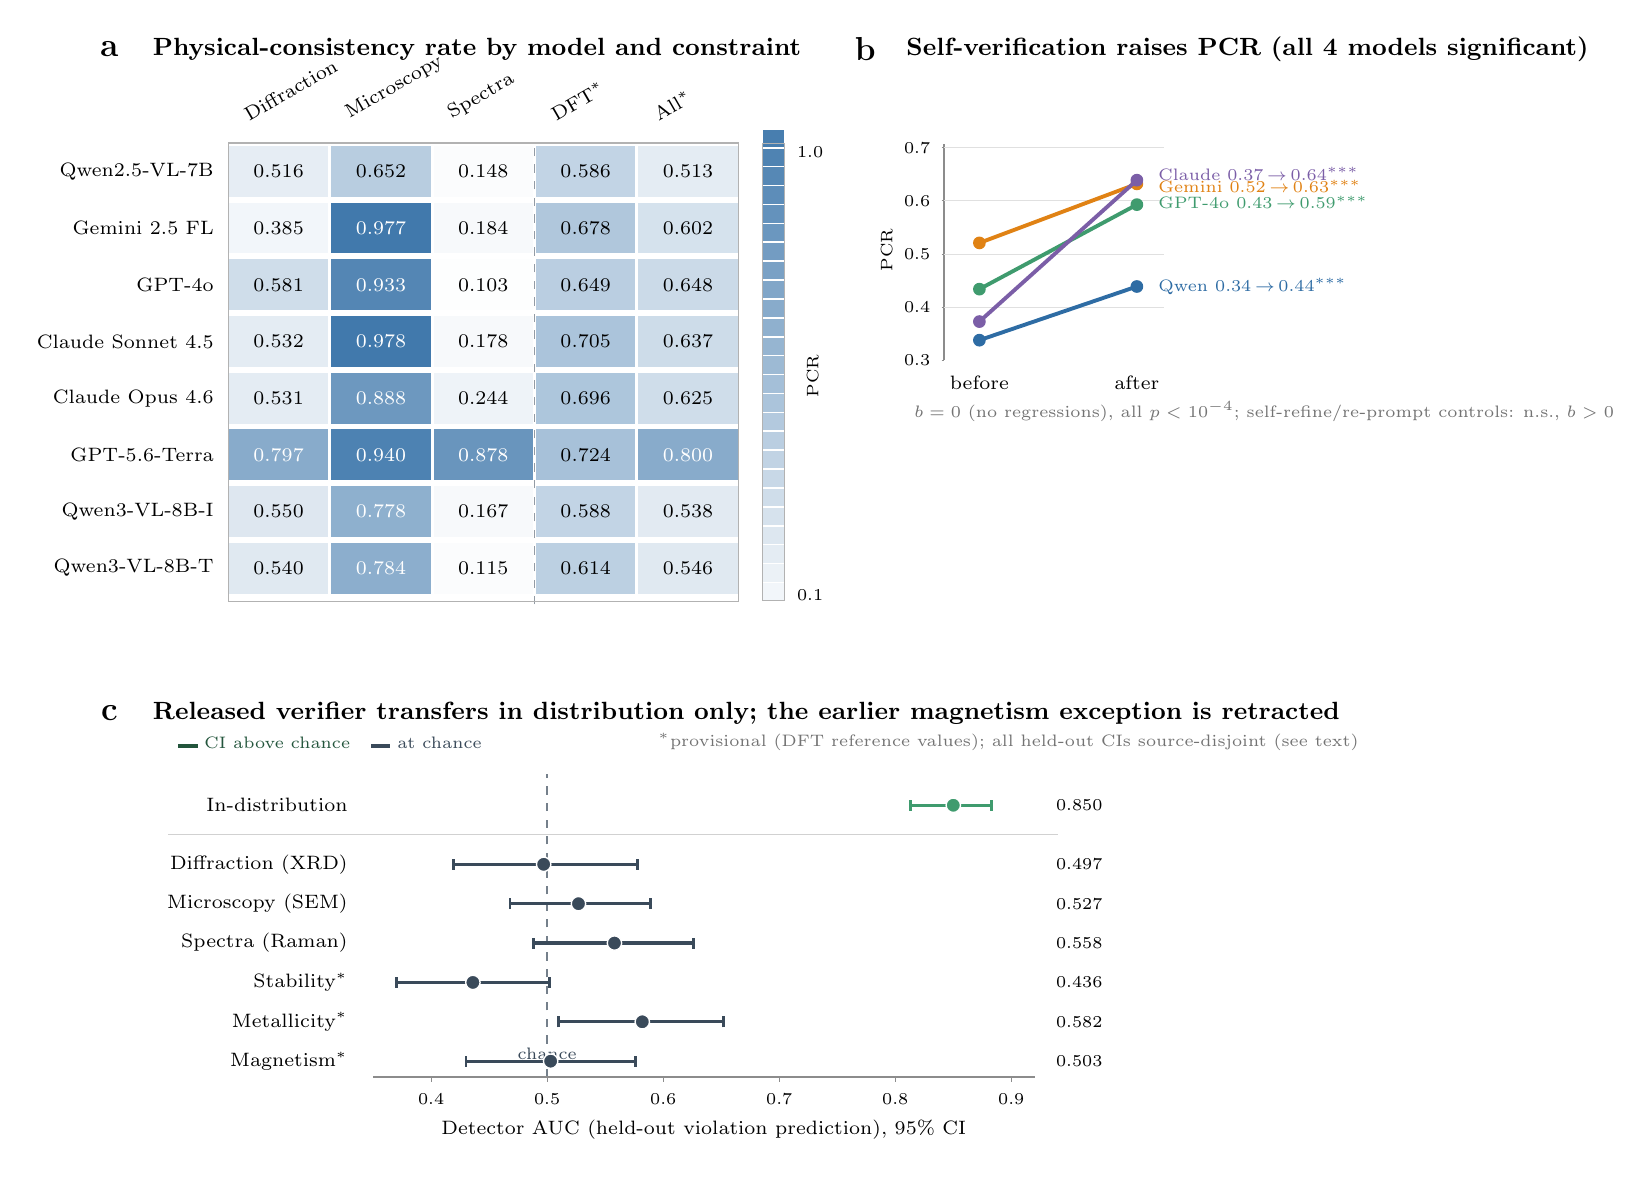
\begin{tikzpicture}[font=\sffamily]

% ---- Panel a: PCR heatmap ----
\node[font=\bfseries\large] at (-0.15,6.65){a};
\node[font=\small\bfseries,anchor=west] at (0.28,6.65){Physical-consistency rate by model and constraint};
\foreach \cx/\lab in {2.0/Diffraction,3.3/Microscopy,4.6/Spectra,5.9/{DFT$^{*}$},7.2/{All$^{*}$}}
  \node[font=\fontsize{6.6}{7}\selectfont,rotate=30,anchor=south west] at (\cx-0.42,5.56){\lab};
\foreach \x/\y/\v/\f/\tc in {%
  2.0/5.10/0.516/12/black, 3.3/5.10/0.652/34/black, 4.6/5.10/0.148/2/black, 5.9/5.10/0.586/29/black, 7.2/5.10/0.513/13/black,
  2.0/4.38/0.385/6/black, 3.3/4.38/0.977/91/white, 4.6/4.38/0.184/4/black, 5.9/4.38/0.678/38/black, 7.2/4.38/0.602/20/black,
  2.0/3.66/0.581/23/black, 3.3/3.66/0.933/82/white, 4.6/3.66/0.103/1/black, 5.9/3.66/0.649/33/black, 7.2/3.66/0.648/25/black,
  2.0/2.94/0.532/13/black, 3.3/2.94/0.978/91/white, 4.6/2.94/0.178/4/black, 5.9/2.94/0.705/40/black, 7.2/2.94/0.637/24/black,
  2.0/2.22/0.531/13/black, 3.3/2.22/0.888/70/white, 4.6/2.22/0.244/8/black, 5.9/2.22/0.696/39/black, 7.2/2.22/0.625/23/black,
  2.0/1.50/0.797/57/white, 3.3/1.50/0.940/85/white, 4.6/1.50/0.878/72/white, 5.9/1.50/0.724/42/black, 7.2/1.50/0.800/57/white,
  2.0/0.78/0.550/16/black, 3.3/0.78/0.778/54/white, 4.6/0.78/0.167/4/black, 5.9/0.78/0.588/29/black, 7.2/0.78/0.538/14/black,
  2.0/0.06/0.540/15/black, 3.3/0.06/0.784/55/white, 4.6/0.06/0.115/2/black, 5.9/0.06/0.614/32/black, 7.2/0.06/0.546/15/black}
  \node[minimum width=1.30cm,minimum height=0.68cm,fill=npblue!\f,draw=white,line width=1pt,inner sep=0,font=\fontsize{7.5}{8}\selectfont,text=\tc] at (\x,\y){\v};
\foreach \y/\lab in {5.10/Qwen2.5-VL-7B,4.38/Gemini 2.5 FL,3.66/GPT-4o,2.94/Claude Sonnet 4.5,2.22/Claude Opus 4.6,1.50/GPT-5.6-Terra,0.78/Qwen3-VL-8B-I,0.06/Qwen3-VL-8B-T}
  \node[font=\fontsize{6.8}{8}\selectfont,anchor=east] at (1.30,\y){\lab};
\draw[npslate!55,dashed,line width=0.5pt] (5.25,-0.40)--(5.25,5.48);
\draw[black!30,line width=0.5pt] (1.36,-0.36) rectangle (7.84,5.46);
\foreach \i in {0,...,24}{\pgfmathsetmacro{\ff}{6+\i*3.4}
  \fill[npblue!\ff] (8.15,-0.35+\i*0.24) rectangle (8.42,-0.13+\i*0.24);}
\draw[black!30,line width=0.4pt](8.15,-0.35) rectangle (8.42,5.45);
\node[font=\fontsize{6}{7}\selectfont,anchor=west] at (8.46,5.35){1.0};
\node[font=\fontsize{6}{7}\selectfont,anchor=west] at (8.46,-0.28){0.1};
\node[font=\fontsize{6}{7}\selectfont,anchor=south,rotate=90] at (8.98,2.5){PCR};

% ---- Panel b: CGSV slopegraph ----
\begin{scope}[shift={(9.9,1.5)}]
\node[font=\bfseries\large] at (-0.45,5.15){b};
\node[font=\small\bfseries,anchor=west] at (-0.05,5.15){Self-verification raises PCR (all 4 models significant)};
\def\yb#1{1.2 + (#1-0.30)/0.40*2.7}
\draw[black!45,line width=0.5pt] (0.55,1.2)--(0.55,3.95);
\foreach \p in {0.3,0.4,0.5,0.6,0.7}{
  \node[font=\fontsize{6}{7}\selectfont,anchor=east] at (0.5,{\yb{\p}}){\p};
  \draw[black!45,line width=0.4pt](0.52,{\yb{\p}})--(0.55,{\yb{\p}});}
\foreach \p in {0.4,0.5,0.6,0.7}\draw[black!12,line width=0.4pt](0.55,{\yb{\p}})--(3.35,{\yb{\p}});
\node[font=\fontsize{6}{7}\selectfont,rotate=90,anchor=south] at (0.02,2.6){PCR};
\node[font=\fontsize{6.6}{8}\selectfont,anchor=north] at (1.0,1.12){before};
\node[font=\fontsize{6.6}{8}\selectfont,anchor=north] at (3.0,1.12){after};
\foreach \a/\c/\col in {0.338/0.439/npblue,0.521/0.632/nporange,0.434/0.593/npgreen,0.373/0.639/nppurple}{
  \draw[\col,line width=1.4pt] (1.0,{\yb{\a}})--(3.0,{\yb{\c}});
  \fill[\col](1.0,{\yb{\a}})circle(2.3pt); \fill[\col](3.0,{\yb{\c}})circle(2.3pt);}
\node[font=\fontsize{6}{7}\selectfont,anchor=west,text=npblue] at (3.15,{\yb{0.439}}){Qwen 0.34\,$\to$\,0.44$^{***}$};
\node[font=\fontsize{6}{7}\selectfont,anchor=west,text=nporange] at (3.15,{\yb{0.632}-0.03}){Gemini 0.52\,$\to$\,0.63$^{***}$};
\node[font=\fontsize{6}{7}\selectfont,anchor=west,text=npgreen] at (3.15,{\yb{0.593}+0.03}){GPT-4o 0.43\,$\to$\,0.59$^{***}$};
\node[font=\fontsize{6}{7}\selectfont,anchor=west,text=nppurple] at (3.15,{\yb{0.639}+0.08}){Claude 0.37\,$\to$\,0.64$^{***}$};
\node[font=\fontsize{5.6}{7}\selectfont,anchor=west,text=black!55] at (0.05,0.55){$b=0$ (no regressions), all $p<10^{-4}$; self-refine/re-prompt controls: n.s., $b>0$};
\end{scope}

% ---- Panel c: verifier AUC forest ----
\begin{scope}[shift={(0,-2.2)}]
\node[font=\bfseries\large] at (-0.15,0.42){c};
\node[font=\small\bfseries,anchor=west] at (0.28,0.42){Released verifier transfers in distribution only; the earlier magnetism exception is retracted};
\def\xa#1{3.2 + (#1-0.35)/0.57*8.4}
\draw[npslate!70,dashed,line width=0.6pt] ({\xa{0.5}},-4.2)--({\xa{0.5}},-0.35);
\node[font=\fontsize{6}{7}\selectfont,text=npslate,anchor=south,fill=white,inner sep=1pt] at ({\xa{0.5}},-4.02){chance};
\draw[black!45,line width=0.5pt] (3.2,-4.2)--(11.6,-4.2);
\foreach \t in {0.4,0.5,0.6,0.7,0.8,0.9}{
  \draw[black!45,line width=0.4pt]({\xa{\t}},-4.2)--({\xa{\t}},-4.27);
  \node[font=\fontsize{6}{7}\selectfont,anchor=north] at ({\xa{\t}},-4.29){\t};}
\node[font=\fontsize{6.8}{8}\selectfont,anchor=north] at (7.4,-4.62){Detector AUC (held-out violation prediction), 95\% CI};
\foreach \y/\lab/\a/\lo/\hi/\col in {%
  -0.75/{In-distribution}/0.850/0.813/0.883/npgreen,
  -1.5/{Diffraction (XRD)}/0.497/0.419/0.578/npslate,
  -2.0/{Microscopy (SEM)}/0.527/0.468/0.589/npslate,
  -2.5/{Spectra (Raman)}/0.558/0.488/0.626/npslate,
  -3.0/{Stability$^{*}$}/0.436/0.370/0.502/npslate,
  -3.5/{Metallicity$^{*}$}/0.582/0.510/0.652/npslate,
  -4.0/{Magnetism$^{*}$}/0.503/0.430/0.576/npslate}{
  \node[font=\fontsize{6.6}{8}\selectfont,anchor=east] at (3.0,\y){\lab};
  \draw[\col,line width=1.2pt]({\xa{\lo}},\y)--({\xa{\hi}},\y);
  \draw[\col,line width=1.0pt]({\xa{\lo}},\y-0.07)--({\xa{\lo}},\y+0.07);
  \draw[\col,line width=1.0pt]({\xa{\hi}},\y-0.07)--({\xa{\hi}},\y+0.07);
  \fill[\col]({\xa{\a}},\y)circle(2.6pt);\draw[white,line width=0.5pt]({\xa{\a}},\y)circle(2.6pt);
  \node[font=\fontsize{6}{7}\selectfont,anchor=west] at (11.75,\y){\a};}
\draw[black!18,line width=0.4pt](0.6,-1.12)--(11.9,-1.12);
\node[font=\fontsize{6}{7}\selectfont,anchor=west,text=npgreen!55!black] at (0.6,0.05){\rule{7pt}{1.6pt}\ CI above chance};
\node[font=\fontsize{6}{7}\selectfont,anchor=west,text=npslate] at (3.05,0.05){\rule{7pt}{1.6pt}\ at chance};
\node[font=\fontsize{6}{7}\selectfont,anchor=west,text=black!55] at (6.7,0.05){$^{*}$provisional (DFT reference values); all held-out CIs source-disjoint (see text)};
\end{scope}

\end{tikzpicture}}
\caption{\textbf{Main results.} \textbf{a}, Physical-Consistency Rate (PCR) for eight
models (four originally evaluated, four current-generation refresh) across four constraint types and overall (Table~\ref{tab:main}), cells shaded by
PCR: microscopy is generally easiest, spectra and diffraction most variable across
models. The
DFT and All columns (asterisk) are provisional pending domain-expert validation.
\textbf{b}, Constraint-Grounded Self-Verification raises PCR from before to after on
identical items (Table~\ref{tab:cgsv}, corrected spectrum oracle); no model regressed a consistent item ($b=0$), and
the increase is significant by the exact paired McNemar test for all four models, unlike
the unaided self-refinement and generic re-prompting controls (both non-significant, both
with $b>0$). \textbf{c}, The released verifier as a
held-out violation detector (Table~\ref{tab:verifier}, source-disjoint split): ROC AUC with bootstrap 95\%
confidence intervals exceeds chance only in distribution; every held-out constraint type,
including magnetism (previously reported as an exception under a since-corrected, leaky
split), is indistinguishable from chance.}
\label{fig:results}
\end{figure}

% =====================================================================
\section*{Discussion}
% =====================================================================
Across eight models spanning two capability generations and six label-free constraint
types, current models are far from
uniformly consistent (overall PCR 0.513--0.800), ruling out the scenario in which the
benchmark would be uninformative because every model already satisfies the physics we
check; spectra and diffraction, in particular, remain hard and highly model-dependent
under the corrected oracles (Methods). Capability scaling within a provider family is not
automatic: the current-generation GPT-5.6-Terra improves clearly over GPT-4o (0.800 vs.\
0.648, non-overlapping bootstrap CIs), but Claude Opus 4.6 does not improve over Claude
Sonnet 4.5, and an explicit reasoning mode (Qwen3-VL-8B-Thinking) does not improve over its
non-reasoning sibling, in this sample. The accuracy-versus-consistency gap (a mean 22.2\% disagreement across 12 cells, revised
downward from an earlier 41.8\% once the spectrum oracle was corrected) shows
directly that PCR is not a restatement of answer accuracy: models are frequently
consistent while measurably wrong on diffraction, and, for stability specifically, frequently correct
by one strict definition while flagged inconsistent by a looser but defensible
tolerance, a real ambiguity in what "stable" should mean for a reasoning check,
not an error in either definition; separately, one model's near-ceiling raw stability
accuracy is a base-rate artifact of the sampled materials, not discriminative skill, once
balanced accuracy is computed. CGSV is a one-directional positive
control: it never regressed a previously consistent item across 545 records, and
raised PCR significantly for all four models tested, an effect two mechanism-isolation
controls (unaided self-refinement, generic equal-compute re-prompting) do not reproduce,
supporting attribution of the gain to the oracle signal rather than to extra
inference-time compute alone. The released verifier is a useful in-distribution
detector (AUC $=0.850$, on a split we rebuilt to be source-disjoint after finding the
original random split leaked item identity across train and test), but its
cross-constraint-type generalization is the paper's clearest
negative result: all six held-out constraint types are indistinguishable from chance.
This corrects an earlier, substantively different finding: under the leaky split, magnetism
appeared to generalize as well held-out as in distribution (AUC $=0.867$); under the
corrected, source-disjoint split, magnetism's held-out AUC is $0.503$, and we now attribute
the earlier result to the split leak rather than to a real transferable signal. We report
this correction, and the resulting simpler and more defensible conclusion (the verifier does
not generalize across constraint types at all), rather than continue to report the
retracted exception, consistent with our stated position that a verifier trained on one
constraint type's surface patterns should not be assumed to transfer to another
without direct evidence. Comparator baselines sharpen this picture: a zero-shot LLM-as-judge
and the model's own token-level self-confidence both perform near or below chance across
splits (Baselines subsection), so the fine-tuned verifier's in-distribution advantage is
real, but it is not a general substitute for the oracle out of distribution. The central limitation is intrinsic to the approach, not
particular to these results: the oracles bound a class of physically checkable
errors, so PCR is a necessary-not-sufficient reliability signal, and the released
verifier predicts the oracle signal rather than replacing first-principles ground
truth. As a clearly scoped extension, the verifier could pre-filter candidate
structures before DFT in a small screening study; a first best-of-3 resampling check finds
real but modest headroom over a random pick (PCR 0.363 random-pick vs.\ 0.419 oracle-oracle
ceiling), though we did not build the verifier-as-selector comparison this ceiling would
need to be practically useful, and report it only as a bounded, partial result. A further implication,
which we make possible but do not claim to demonstrate here, is that a label-free,
physics-grounded consistency signal can serve as a verifiable reward for training
materials-reasoning models, extending reinforcement learning from verifiable rewards
to a domain where verification has been under-specified.\cite{scirlvr2026} We also ran a
domain-specific structure-aware model (MatterChat) on the DFT arms as a materials-domain
evaluee (Baselines subsection): it reaches PCR 0.783/0.795/0.850 on stability/metallicity/
magnetism on a shuffled sample of 120 real materials, comparable to or better than the
general-purpose models on the same arms, though this is a single domain model on one
sample and we do not generalize beyond it. Finally,
every DFT-grounded number in this paper (the DFT column of Table~\ref{tab:main}, the
stability arm of the accuracy-versus-consistency analysis, and the metallicity and
magnetism arms of the verifier and detector analyses) rests on Materials Project
reference values and oracle tolerances that have not yet been independently reviewed
by the domain co-author; we report them as measured and provisional, and will revise
or withdraw any claim that review does not support before final submission.

% =====================================================================
\section*{Methods}
% =====================================================================
\subsection*{Data sources}
MatPCR draws only on public data for reproducibility and license clarity: simulated
and experimental powder diffraction with known structures;\cite{simxrd2024,opxrd2025}
public SEM/TEM corpora that include scale bars;\cite{aversa2018nffa} open Raman and
infrared spectra;\cite{lafuente2015rruff} and public first-principles data (computed
energies, convex hulls, band gaps) from established databases,\cite{matproj2013}
supplemented by the authors' own DFT where a reference value is required.

\subsection*{Tasks, modalities, and exposed constraints}
Each item pairs an input with a question whose faithful answer requires at least one
physically checkable quantity. Inputs span image items (VLM), such as micrographs and
diffraction images, and structure or text items (LLM), such as a crystal structure
with a property question. We parse the reasoning chain for stated quantities (peak
positions, scale, feature sizes, stability claims, property values) and test each
against the matching oracle. An item is checkable if its chain exposes at least one
such quantity.

\subsection*{Programmatic geometric oracles}
For diffraction we apply Bragg's law, $\lambda = 2 d \sin\theta$, converting any
claimed $2\theta$ to a $d$-spacing, testing claimed peaks against the reference
pattern of the stated structure within tolerance, and rejecting claims outside the
realizable $2\theta$ window. For microscopy we recover nanometres per pixel from the
detected scale bar and reject any feature larger than the field of view. For spectra
we accept a claimed peak only if a genuine interior local maximum (higher than both
adjacent flanks down to their nearest valleys, rejecting a monotonic rise or a shoulder on
a nearby peak) exists near it with prominence exceeding a fraction of the signal's dynamic
range; this is a revision, made mid-project after a first precision audit showed a
windowed-maximum check without the interior-local-maximum requirement was too permissive
on noisy, baseline-drifting Raman spectra, so it does not appear in numbers computed
before the revision (flagged where relevant throughout).

\subsection*{DFT-grounded property oracles}
First-principles access extends the oracle from geometry to computed physics, still
without human labels. A stability claim is checked against the energy above the
convex hull computed for the stated composition; a metallicity claim against the
computed band gap; and a magnetism claim against the computed total magnetization,
normalized per atom. Reference values are Materials Project's own standardized
computational references (database version 2026.04.13, retrieved 2026-07-16 via the
\texttt{mp-api} client; GGA/GGA+U relaxation under Materials Project's published standard
workflow), described throughout as standardized computational references, not
experimental ground truth, per the domain co-author's guidance; the authors' own DFT is
reserved for missing or questionable cases and was not run over the full sample reported
here. Because DFT-computed
references depend on the exchange-correlation functional (semilocal functionals
underestimate band gaps), each oracle is designed around that known error rather than
treating the reference as exact. \emph{Stability}: a claim is consistent iff the claimed
stable/unstable label agrees with whether the computed energy above the convex hull is
within a tolerance $\epsilon=0.05\,\mathrm{eV\,atom^{-1}}$ of the hull; we additionally
report sensitivity at $\epsilon\in\{0,0.025,0.05,0.10\}\,\mathrm{eV\,atom^{-1}}$ (all four
gave 0\% false-negative and false-positive rates in the positive-control audit), and, per
the domain co-author's review, structures with $0<\epsilon\le0.05$ are described as
near-hull or potentially metastable, never as strictly stable. \emph{Metallicity}: a
computed band gap $\le0.05\,\mathrm{eV}$ is treated as computed-metallic,
$\ge0.20\,\mathrm{eV}$ as computed-non-metallic, and the intervening band
($0.05$--$0.20\,\mathrm{eV}$) is an explicit abstention band excluded from PCR rather than
forced into either class, both thresholds the domain co-author's literal recommendation.
\emph{Magnetism}: total magnetization is conventionally nonnegative in a DFT calculation
and can flip sign under an arbitrary global spin-reversal choice, so it is never treated as
a signed quantity; the reference is normalized to $|{\rm total\ magnetization}|$ per atom,
classified magnetic versus non-magnetic at a preregistered threshold of
$0.05\,\mu_{\rm B}\,{\rm atom}^{-1}$, and, only within the magnetic class, a claimed
magnitude is checked against the reference within one order of magnitude; a near-zero
reference is treated as zero within an absolute tolerance of $10^{-6}\,\mu_{\rm B}$ (see
below) rather than by exact floating-point equality. Positive-control testing showed all
three thresholds and the stability sensitivity grid give 0\% false-negative and
false-positive rates on real Materials Project structures; the metallicity abstention band
correctly excluded 125 of 3{,}000 sampled materials in that test. These checks make plausible-but-wrong physics detectable.
No step requires a human annotation of the correct answer, which is what lets MatPCR
scale and distinguishes it from answer-accuracy benchmarks and from proposal- or
execution-level verification.

\subsection*{The Physical-Consistency Rate}
Let items be indexed $i=1,\dots,N$, let $k_i$ be the number of physically checkable
constraints the chain exposes on item $i$, and $v_i \le k_i$ the number the oracles
find violated. The item is consistent iff $v_i=0$. Over the checkable subset
$\mathcal{C}=\{i:k_i>0\}$,
\begin{equation}
\mathrm{PCR} \;=\; \frac{1}{|\mathcal{C}|}\sum_{i\in\mathcal{C}} \mathbf{1}[v_i = 0].
\end{equation}
We report per-constraint-type violation rates
$\rho_t=\big(\sum_i v_{i,t}\big)/\big(\sum_i k_{i,t}\big)$ and per-modality rates with
percentile bootstrap confidence intervals. PCR is distinct from answer accuracy: a
model can be accurate yet inconsistent, or consistent yet wrong, and the gap is
itself reported.

\subsection*{Constraint-Grounded Self-Verification}
CGSV uses the same oracles as a corrective signal at inference time with no labels.
Because a model's own self-verification is largely confirmatory rather than
corrective,\cite{selfverify2026} CGSV supplies the correction signal externally, from the
oracle, rather than asking the model to re-examine its answer unaided. The model extracts
the governing constraints, answers, is shown any programmatic or DFT-grounded violation,
and revises, up to $K$ rounds or until no violation remains (Algorithm~\ref{alg:cgsv}).
CGSV is a positive control: if the oracles capture real errors, exposing them should raise
PCR, measured by a paired test, not assumed.

\begin{algorithm}[t]
\caption{Constraint-Grounded Self-Verification}
\label{alg:cgsv}
\begin{algorithmic}[1]
\State \textbf{Input:} input $x$, question $q$, oracle set $\mathcal{O}$, max rounds $K$
\State $G \gets \textsc{ExtractConstraints}(x)$
\State $a \gets \textsc{Answer}(x,q,G)$
\For{$r = 1 \dots K$}
  \State $V \gets \{o \in \mathcal{O} : o(\textsc{Claims}(a), G)\ \text{fails}\}$
  \If{$V = \varnothing$} \State \textbf{break} \EndIf
  \State $a \gets \textsc{Revise}(x, q, G, a, V)$
\EndFor
\State \textbf{return} $a$, residual violations $V$
\end{algorithmic}
\end{algorithm}

\subsection*{Released physical-consistency verifier}
Because the oracles require reference data (a structure, a scale bar, a computed
value), we fine-tune an open model to predict, from the input and chain alone,
whether a physical violation is present. Training labels come from the oracles, so the
verifier is trained without human annotation. Unlike process-reward and generative
reward models trained on human preference or model-judged
correctness,\cite{processbench2025,compassverifier2025} its labels are a deterministic
physics signal, which reduces the spurious correlations that affect preference-trained
reward models; where a reference exists, the oracle is hard to game by surface-form changes. We release it as the reusable artifact of this work and report precision,
recall, $F_1$, ROC AUC, and calibration against held-out oracle judgments.

% Figure 2: pipeline
\begin{figure}[t]
\centering
\resizebox{\linewidth}{!}{%
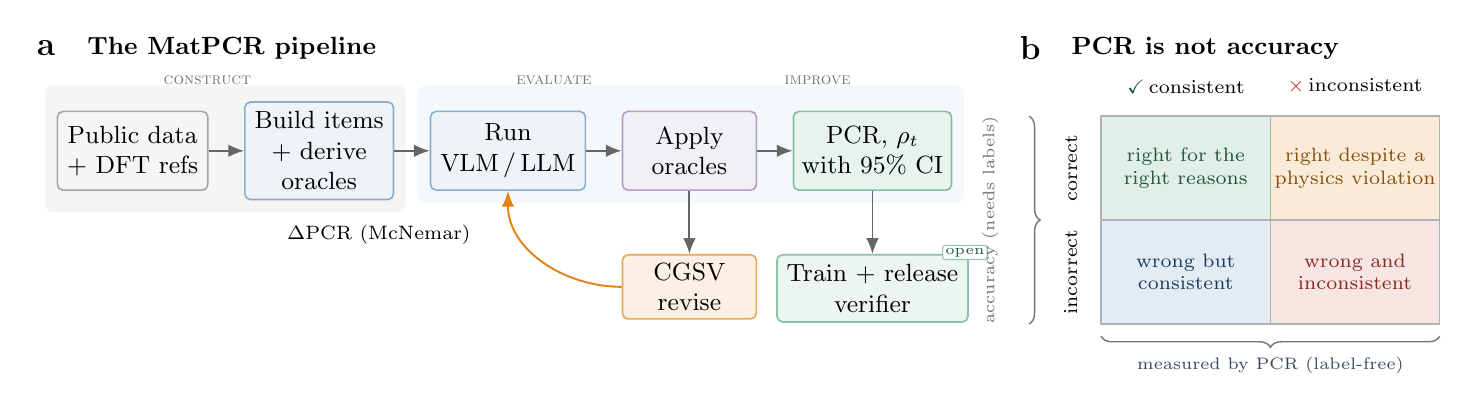
\begin{tikzpicture}[font=\sffamily]
\node[plab] at (-0.1,2.55){a};
\node[font=\small\bfseries,anchor=west] at (0.3,2.55){The MatPCR pipeline};

% phase labels
\node[font=\fontsize{6.5}{8}\selectfont,black!55] at (1.95,2.15){\textsc{construct}};
\node[font=\fontsize{6.5}{8}\selectfont,black!55] at (6.35,2.15){\textsc{evaluate}};
\node[font=\fontsize{6.5}{8}\selectfont,black!55] at (9.7,2.15){\textsc{improve}};

\node[data,minimum width=1.7cm,minimum height=1.0cm] (pub) at (1.0,1.25){Public data\\+ DFT refs};
\node[proc,right=4.5mm of pub,minimum width=1.7cm,minimum height=1.0cm] (build){Build items\\+ derive\\oracles};
\node[proc,right=4.5mm of build,minimum width=1.7cm,minimum height=1.0cm] (run){Run\\VLM\,/\,LLM};
\node[proc,right=4.5mm of run,fill=nppurple!10,draw=nppurple!60,minimum width=1.7cm,minimum height=1.0cm] (chk){Apply\\oracles};
\node[good,right=4.5mm of chk,minimum width=1.85cm,minimum height=1.0cm] (pcr){PCR, $\rho_t$\\with 95\% CI};

% faint phase bands
\begin{scope}[on background layer]
  \fill[black!4,rounded corners=3pt] ($(pub.north west)+(-0.15,0.32)$) rectangle ($(build.south east)+(0.15,-0.15)$);
  \fill[npblue!5,rounded corners=3pt] ($(run.north west)+(-0.15,0.32)$) rectangle ($(pcr.south east)+(0.15,-0.15)$);
\end{scope}

\draw[flow](pub)--(build);\draw[flow](build)--(run);\draw[flow](run)--(chk);\draw[flow](chk)--(pcr);
\node[acc,below=8mm of chk,minimum width=1.7cm] (cgsv){CGSV\\revise};
\node[proc,below=8mm of pcr,fill=npgreen!10,draw=npgreen!60,minimum width=1.85cm] (ver){Train + release\\verifier};
\node[font=\fontsize{5.5}{6}\selectfont,npgreen!55!black,fill=white,draw=npgreen!55,rounded corners=1pt,inner sep=1pt] at ($(ver.north east)+(-0.05,0.02)$){open};
\draw[flow](chk.south)--(cgsv.north);
\draw[flow,nporange](cgsv.west) to[out=180,in=-90] (run.south);
\node[font=\scriptsize,black,anchor=east] at ($(run.south)+(-0.35,-0.55)$) {$\Delta$PCR (McNemar)};
\draw[flow](pcr.south)--(ver.north);

% ---- Panel b: 2x2 ----
\node[plab] at (12.4,2.55){b};
\node[font=\small\bfseries,anchor=west] at (12.8,2.55){PCR is not accuracy};

\begin{scope}[shift={(13.3,-0.95)}]
  \def\cw{2.15}\def\ch{1.32}
  \fill[npgreen!16](0,\ch) rectangle (\cw,2*\ch);
  \fill[nporange!16](\cw,\ch) rectangle (2*\cw,2*\ch);
  \fill[npblue!13](0,0) rectangle (\cw,\ch);
  \fill[npred!13](\cw,0) rectangle (2*\cw,\ch);
  \draw[black!30,line width=0.5pt](0,0) rectangle (2*\cw,2*\ch);
  \draw[black!30,line width=0.5pt](\cw,0)--(\cw,2*\ch);
  \draw[black!30,line width=0.5pt](0,\ch)--(2*\cw,\ch);
  \node[align=center,font=\scriptsize,text=npgreen!55!black] at (0.5*\cw,1.5*\ch){right for the\\right reasons};
  \node[align=center,font=\scriptsize,text=nporange!60!black] at (1.5*\cw,1.5*\ch){right despite a\\physics violation};
  \node[align=center,font=\scriptsize,text=npblue!55!black] at (0.5*\cw,0.5*\ch){wrong but\\consistent};
  \node[align=center,font=\scriptsize,text=npred!70!black] at (1.5*\cw,0.5*\ch){wrong and\\inconsistent};
  % column headers with icons
  \node[font=\scriptsize,anchor=south] at (0.5*\cw,2*\ch+0.16){\textcolor{npgreen!60!black}{\checkmark}\,consistent};
  \node[font=\scriptsize,anchor=south] at (1.5*\cw,2*\ch+0.16){\textcolor{npred}{$\times$}\,inconsistent};
  % row headers
  \node[font=\scriptsize,rotate=90,anchor=south] at (-0.18,1.5*\ch){correct};
  \node[font=\scriptsize,rotate=90,anchor=south] at (-0.18,0.5*\ch){incorrect};
  % braces
  \draw[decorate,decoration={brace,amplitude=4pt,mirror,raise=1pt},black!55,line width=0.5pt]
     (0,-0.12)--(2*\cw,-0.12);
  \node[font=\fontsize{6.5}{8}\selectfont,anchor=north,text=npslate] at (\cw,-0.30){measured by PCR (label-free)};
  \draw[decorate,decoration={brace,amplitude=4pt,raise=1pt},black!55,line width=0.5pt]
     (-0.95,2*\ch)--(-0.95,0);
  \node[font=\fontsize{6.5}{8}\selectfont,rotate=90,anchor=south,text=black!55] at (-1.18,\ch){accuracy (needs labels)};
\end{scope}
\end{tikzpicture}}
\caption{\textbf{The MatPCR framework.} \textbf{a}, Across the construct, evaluate and improve phases, items and oracles are built from public data and density-functional-theory references; reasoning chains are scored to produce the Physical-Consistency Rate (PCR) and per-constraint-type violation rates $\rho_t$ with bootstrap confidence intervals; oracle judgments train a released verifier and drive CGSV, whose effect on PCR is quantified by a paired McNemar test. \textbf{b}, PCR is distinct from answer accuracy: a chain can be right for the right reasons, right despite a physics violation, wrong but physically consistent, or wrong and inconsistent. Accuracy resolves the rows (and needs labels); MatPCR resolves the columns, the consistency axis, without labels.}
\label{fig:pipeline}
\end{figure}

\subsection*{Measurement guarantees}
We give exact, assumption-light guarantees relating the \emph{measured} PCR to the
\emph{true} physical-consistency rate, decomposing the reported estimate's error into an
oracle-bias term and a sampling term, and we quantify the effect of an imperfect
oracle, of CGSV, and of substituting the learned verifier for the oracle. Let
$\mathcal{C}$ be the set of checkable items with $|\mathcal{C}|=n$, where here $n$ denotes
the number of checkable items in the set under analysis (distinct from the per-cell item
count of the evaluation tables). For
$i\in\mathcal{C}$ let $Y_i\in\{0,1\}$ be the latent indicator that the chain contains
at least one genuine physical violation and $\hat Y_i\in\{0,1\}$ the oracle's decision.
The true inconsistency rate is $\tau=\frac1n\sum_i Y_i$, the true rate is
$\mathrm{PCR}^\star=1-\tau$, and the measured rate is
$\mathrm{PCR}=1-\frac1n\sum_i\hat Y_i$. Define the empirical item-level recall and
false-alarm rate of the oracle,
$\hat d=\#\{\hat Y_i{=}1,Y_i{=}1\}/\#\{Y_i{=}1\}$ and
$\hat f=\#\{\hat Y_i{=}1,Y_i{=}0\}/\#\{Y_i{=}0\}$ (a rate multiplies a zero
count to zero when its class is empty).

\begin{proposition}[Bias decomposition]\label{prop:bias}
$\mathrm{PCR}-\mathrm{PCR}^\star=\tau(1-\hat d)-(1-\tau)\hat f.$
\end{proposition}
\begin{proof}
Counting flagged items,
$\sum_i\hat Y_i=\hat d\,\#\{Y_i{=}1\}+\hat f\,\#\{Y_i{=}0\}=n[\tau\hat d+(1-\tau)\hat f]$,
so $\mathrm{PCR}=1-\tau\hat d-(1-\tau)\hat f$. Subtracting $\mathrm{PCR}^\star=1-\tau$
gives the result.
\end{proof}

\begin{corollary}[One-sided guarantees and bias bound]\label{cor:onesided}
If the oracle is complete $(\hat d=1)$ then $\mathrm{PCR}\le\mathrm{PCR}^\star$, so PCR
never overstates consistency; if it is sound $(\hat f=0)$ then
$\mathrm{PCR}\ge\mathrm{PCR}^\star$; if both, $\mathrm{PCR}=\mathrm{PCR}^\star$. In
general $|\mathrm{PCR}-\mathrm{PCR}^\star|\le(1-\hat d)+\hat f$.
\end{corollary}
\begin{proof}
The three cases substitute $\hat d=1$ and $\hat f=0$ into
Proposition~\ref{prop:bias}. For the bound,
$|\tau(1-\hat d)-(1-\tau)\hat f|\le\tau(1-\hat d)+(1-\tau)\hat f\le(1-\hat d)+\hat f$
because $\tau,\,1-\tau\le1$.
\end{proof}

\noindent Corollary~\ref{cor:onesided} is the formal reason to run the positive control
and precision audit first (Table~\ref{tab:exp1}). The positive control estimates the
oracle's recall $\hat d$ (planted-violation recovery). The precision audit estimates its
precision $\pi$ on fired cases, equivalently the false-discovery rate $1-\pi$; this is not
the false-alarm rate $\hat f$, whose denominator is the truly-clean items, and the two
coincide only through the base rate. Under the $\hat d=1$ idealization supported by the
positive control, Corollary~\ref{cor:onesided} gives $\mathrm{PCR}\le\mathrm{PCR}^\star$,
and the understatement is exactly the false-positive fraction $(1-\pi)(1-\mathrm{PCR})$, which the
audited precision estimates directly; estimating $\hat f$ itself, and hence the bias when
$\hat d<1$, additionally requires sampling oracle-silent items to fix the base rate.

Proposition~\ref{prop:bias} and Corollary~\ref{cor:onesided} concern the oracle bias on
a fixed set of items. The reported PCR is also a finite sample, so its error as an
estimate of the underlying consistency rate has a second, statistical part, which the
next result bounds together with the bias.

\begin{proposition}[Total error of the reported estimate]\label{prop:total}
Suppose the checkable items are drawn independently from the benchmark's item-generating
process and let $\mu=\mathbb{E}[1-Y_i]$ be that process's physical-consistency rate. For
any $t>0$, with probability at least $1-2e^{-2nt^2}$ over the sampling,
\begin{equation*}
|\mathrm{PCR}-\mu|\;\le\;\underbrace{(1-\hat d)+\hat f}_{\text{oracle bias}}\;+\;\underbrace{t}_{\text{sampling}} .
\end{equation*}
When items share a parent source, the analogous bound holds with $n$ replaced by the
number $m$ of independent sources under balanced source sizes (unequal sizes give a
size-weighted mean and a correspondingly weakened rate).
\end{proposition}
\begin{proof}
Split $\mathrm{PCR}-\mu=(\mathrm{PCR}-\mathrm{PCR}^\star)+(\mathrm{PCR}^\star-\mu)$.
Corollary~\ref{cor:onesided} bounds the first term by $(1-\hat d)+\hat f$. The second,
$\mathrm{PCR}^\star=\frac1n\sum_i(1-Y_i)$, is a mean of independent $[0,1]$ variables with
expectation $\mu$, so Hoeffding's inequality (Appendix~\ref{app:concentration}) gives
$\Pr[|\mathrm{PCR}^\star-\mu|>t]\le 2e^{-2nt^2}$; the triangle inequality combines the two,
and grouping by balanced sources replaces $n$ with the source count $m$.
\end{proof}

\noindent The independence assumption is an idealization for a convenience benchmark;
source-level grouping relaxes it to independent sources. Both terms are separately
estimated and reported: the oracle bias from the positive control and precision audit
(Table~\ref{tab:exp1}, and the base-rate caveat above), and the sampling term by the
percentile bootstrap interval (Appendix~\ref{app:standard}), under the idealization that
the oracle's gate-estimated error rates transfer to the evaluation items.
Proposition~\ref{prop:total} is the sense in which a reported PCR bounds the true
consistency rate, not only the sampled chains.

\begin{proposition}[CGSV accounting and termination]\label{prop:cgsv}
Let $c$ and $b$ be the numbers of items the oracle flags before but not after CGSV
(fixes) and after but not before (regressions), respectively. Then
$\Delta\mathrm{PCR}=(c-b)/n$, and the loop halts within $K$ rounds. If, in addition,
no revision enlarges an item's oracle-violation set (Assumption~A), then $b=0$ and
$\Delta\mathrm{PCR}\ge0$.
\end{proposition}
\begin{proof}
With per-item consistency indicators $s_i^{(0)}=1-\hat Y_i^{(0)}$ before CGSV and
$s_i^{(1)}=1-\hat Y_i^{(1)}$ after, $\Delta\mathrm{PCR}=\frac1n\sum_i(s_i^{(1)}-s_i^{(0)})$;
each summand is $+1$ on a fix, $-1$ on a regression, and $0$ otherwise, summing to
$(c-b)/n$. Termination is immediate from the bounded loop. Under Assumption~A,
$\hat Y_i^{(1)}\le\hat Y_i^{(0)}$ for all $i$, so $b=0$.
\end{proof}

\noindent We do not assume Assumption~A holds; the exact McNemar test on the discordant
pair $(b,c)$ tests the null that a changed item is equally likely to be a fix or a
regression, namely $c\sim\mathrm{Binomial}(b+c,\tfrac12)$ (Appendix).

\begin{proposition}[Verifier substitution]\label{prop:verifier}
Let $\hat Y^o$ and $\hat Y^v$ be the oracle and verifier decisions and
$\delta=\frac1n\#\{i:\hat Y^v_i\neq\hat Y^o_i\}$ their disagreement rate. Then
$|\mathrm{PCR}^v-\mathrm{PCR}^o|\le\delta$ and hence
$|\mathrm{PCR}^v-\mathrm{PCR}^\star|\le(1-\hat d)+\hat f+\delta$.
\end{proposition}
\begin{proof}
$|\mathrm{PCR}^v-\mathrm{PCR}^o|=\big|\frac1n\sum_i(\hat Y^o_i-\hat Y^v_i)\big|
\le\frac1n\sum_i|\hat Y^o_i-\hat Y^v_i|=\delta$. Combining with
Corollary~\ref{cor:onesided} by the triangle inequality gives the second bound.
\end{proof}

\noindent These bounds make the verifier usable when reference data are unavailable at
inference: its PCR estimates inherit the oracle's guarantees up to the measurable
disagreement $\delta$, the verifier's error rate against the oracle labels that its
precision and recall in Table~\ref{tab:verifier} summarize. Because that disagreement is
small only in distribution and large where transfer fails, the bound is tight in
distribution and loose out of it, which is exactly where reference data are absent; we
therefore present it as a guarantee for in-distribution use, not a license to replace the
oracle across constraint types. Standard background results
(Bragg's law, scale-bar calibration, convex-hull stability, the percentile bootstrap, a
concentration inequality for the empirical rate, and the exact McNemar test) are
collected in the Appendix.

\subsection*{Models and experimental protocol}
We evaluate eight models in total across two passes. The original pass (data collected
2026-07-04 through 2026-07-11, re-run on corrected oracles 2026-07-16/17) covers one open
vision--language model, Qwen2.5-VL-7B-Instruct\cite{qwen25vl} (Hugging Face repository
\texttt{Qwen/Qwen2.5-VL-7B-Instruct}, run locally in \texttt{bfloat16} on an NVIDIA A100
80GB via \texttt{transformers}), and three frontier models accessed through the OpenRouter
API: \texttt{openai/gpt-4o}, \texttt{google/gemini-2.5-flash-lite}, and
\texttt{anthropic/claude-sonnet-4.5}. A current-generation refresh pass (data collected
2026-07-19/20) adds \texttt{anthropic/claude-opus-4.6}, \texttt{openai/gpt-5.6-terra},
\texttt{qwen/qwen3-vl-8b-instruct}, and a reasoning-mode condition,
\texttt{qwen/qwen3-vl-8b-thinking}, all four again via OpenRouter. Model strings, weights, and
API routing are pinned in the released repository; OpenRouter does not expose a
per-request snapshot date distinct from the model string for these providers, so the
listed model identifiers and the stated collection dates are the reproducibility anchor. We additionally evaluate a materials-domain
structure-aware model, MatterChat\cite{matterchat2026} (its released Mistral-7B-based
checkpoint and CHGNet structure encoder, run locally), on the DFT arms only (Baselines
subsection); no LLaVA-class model was run, and that mention is removed below.

For each model and item we sample reasoning chains at a fixed decoding configuration
with $S=3$ seeds, apply the oracles, and report mean PCR with percentile bootstrap
confidence intervals ($B=10{,}000$ resamples); CGSV uses the same decoding and $K=2$
rounds. The local model uses greedy decoding (\texttt{do\_sample=False}); the API models
are called with no explicit temperature or top-$p$ override, i.e.\ each provider's own
default sampling settings for the given model string, which we did not tune. We ran the most informative experiment first, the
oracle-validity gate reported above (Table~\ref{tab:exp1}): a positive control that
injected synthetic violations into otherwise valid chains at known rates and confirmed
the oracles recover them, followed by a manual audit of oracle-fired cases that
quantified oracle precision on real chains. This established that PCR measures genuine
physical violations rather than parsing artifacts. Tolerances, prompts, and the DFT
protocol are pre-registered and released; we report $S=3$ seeds per condition, bootstrap
confidence intervals on all rates, and the exact McNemar test for paired before/after
comparisons. Each seed draws a fresh, independently sampled subset of items (verified
directly: zero duplicate source files across seeds in every (constraint-type, model) cell
checked), so the $S=3$ seeds are not the same items re-scored, and pooling records across
seeds within a cell does not pool literal duplicates. This does not, however, resolve the
separate, still-open concern that the full sweep runs $8\times6\times3=144$ (model,
constraint-type, seed) cells and 4 CGSV comparisons without a multiple-comparisons
correction (Baselines subsection, Statistics paragraph); that correction has not yet been
applied and every reported $p$-value below should be read as uncorrected for the family of
tests it belongs to.

\subsection*{Baselines, ablations, and controls}
Three of the study's controls are stronger than those reported in several comparable
verifier and reasoning-benchmark studies: the oracle positive control with a precision
audit, bootstrap confidence intervals with an exact paired test, and a held-out-constraint
generalization split.
% VERIFY at submission that the closest neighbors indeed omit these controls.
A physical-consistency metric, a released verifier, and a self-correction loop are
nonetheless interpretable only against the further baselines and controls specified here;
those not yet reported are flagged for completion before submission.

\noindent\emph{Models.} We added the current-generation refresh and reasoning-mode
condition described above (Claude Opus 4.6, GPT-5.6-Terra, Qwen3-VL-8B-Instruct,
Qwen3-VL-8B-Thinking), and a materials-domain evaluee. For the domain evaluee we ran
MatterChat\cite{matterchat2026}, a structure-aware model that aligns a pretrained CHGNet
material encoder with a Mistral-7B language model, on the three DFT constraint types (its
native input, a crystal structure) using its released checkpoint and code, on a shuffled
sample of 120 real Materials Project structures (an unshuffled first sample, drawn in raw
file order, was 3.3\% magnetic versus the corrected sample's 65\%, so we discarded it and
redrew with shuffling before reporting). MatterChat reaches PCR 0.783 (stability), 0.795
(metallicity, $n=112$ checkable of 120), and 0.850 (magnetism, genuinely varying its answer
across materials rather than defaulting to one class, confirmed directly). We did not run a
domain-specific model on the image arms (no comparably released microscopy-specific VLM was
identified). On reasoning mode: Qwen3-VL-8B-Thinking does not improve over
Qwen3-VL-8B-Instruct overall (0.546 vs.\ 0.538, bootstrap CIs overlapping), so explicit
reasoning mode alone does not reliably raise PCR in this sample (Results).

\noindent\emph{Verifier baselines.} We compare the released verifier against a zero-shot
LLM-as-judge (Gemini 2.5 Flash Lite, prompted to judge each chain for a physical-consistency
violation with a stated confidence) and the evaluated local model's own token-level
self-confidence (mean log-probability of its stated final answer span), on the same
in-distribution and six held-out-constraint-type splits, 2{,}152 items. Neither baseline
is competitive with the fine-tuned verifier in distribution: the LLM-judge reaches
AUC $=0.447$ (95\% CI $[0.400,0.493]$, indistinguishable from or below chance) and
self-confidence AUC $=0.315$ (95\% CI $[0.264,0.365]$, significantly \emph{below} chance,
an anti-correlation we discuss below), against the fine-tuned verifier's in-distribution
AUC $=0.850$. Held out, all three approaches are weak: the LLM-judge ranges AUC
$0.489$--$0.735$ across the six constraint types (best on microscopy, worst on diffraction)
and self-confidence ranges AUC $0.246$--$0.523$, several below chance; neither baseline
recovers the fine-tuned verifier's in-distribution advantage out of distribution, and
none of the three approaches is a reliable held-out detector. We investigated the
below-chance self-confidence result directly rather than treat it as noise: on a 40-item
sample, chains later judged physically inconsistent had a \emph{higher} mean token
log-probability ($-2.84$) than chains judged consistent ($-3.99$), i.e.\ the evaluated
model is more confident, not less, when it is physically wrong, which is the source of the
below-chance AUC rather than a sign error in our scoring. We separately built reliability
diagrams (binned calibration curves) and a recommended per-split operating threshold for
the released verifier: in distribution its predicted probabilities are reasonably
calibrated (seven of ten reliability bins have a gap under 0.1 between predicted and
empirical violation rate; the two largest gaps are 0.198 in the 0.1--0.2 bin and 0.228 in
the 0.3--0.4 bin) and its default 0.5 threshold is close to optimal (best $F_1=0.765$ at threshold
0.25 versus $F_1=0.735$ at 0.5). Held out, however, every constraint type is severely
miscalibrated in the same direction: the verifier's low-probability bins massively
underestimate the true violation rate (for example, held-out diffraction: predicted
$0.07$--$0.14$ in its lowest bins, actual $0.47$--$0.49$; held-out spectra: predicted
$0.02$--$0.15$, actual $0.84$--$0.93$), so at the default 0.5 threshold the verifier
essentially never fires held out (recall as low as 0.03 for diffraction), and a much lower
threshold (0.05 in five of six held-out splits) recovers usable recall at a real precision
cost (for example, held-out diffraction $F_1$ rises from 0.057 at threshold 0.5 to 0.628 at
threshold 0.05). No off-the-shelf process-reward model (PRM) comparison is reported: we
checked directly and found no general-purpose or physics/materials-science PRM publicly
available; every widely used open PRM (for example Qwen2.5-Math-PRM-7B, PRM800K-tuned
variants, MedPRM) is trained on a specific domain's own step-labeled data (mathematics,
medicine), so applying one to these physics reasoning chains would be an uninterpretable
domain mismatch rather than a meaningful comparator, and we report this as a genuine
absence rather than an oversight.

\noindent\emph{Self-verification controls.} We isolate CGSV's contribution with three
controls, matched to CGSV's items, models, $K$, and decoding: (i) unaided
self-refinement, in which the model is told only to double-check its answer with no oracle
feedback, shows no significant change (PCR $0.349\to0.339$, $n=542$, $b=34$, $c=29$,
$p=0.615$); (ii) generic equal-compute re-prompting, in which the model is simply asked to
reconsider with no critique framing, likewise shows no significant change
($0.358\to0.342$, $n=562$, $b=24$, $c=15$, $p=0.20$); both controls, unlike CGSV, show
nonzero regressions. (iii) Best-of-3 independent resampling (no multi-turn revision) gives a
random-pick PCR of $0.363$ and an oracle-oracle best-of-3 ceiling of $0.419$ ($n=614$),
both well below CGSV's after-PCR for every model. We did not build a verifier-as-selector
comparison on top of best-of-$N$ (this would need each candidate's chain text persisted for
verifier scoring, which the current best-of-$N$ harness does not retain), so the
best-of-3 result establishes only that resampling alone leaves real headroom over a random
pick, not that the verifier can currently capture it; this is reported as a partial result. Together, CGSV's significant, zero-regression gain
against two null controls supports attributing it to the physical-consistency signal
specifically, not to generic self-reflection or additional sampling at equal compute
(Results, CGSV table).

\noindent\emph{Ablations, human agreement, and error analysis.} (i) Tolerance sensitivity:
we re-checked already-collected real model claims against the oracle at multiple tolerance
settings without new model calls. Diffraction's model ranking is \emph{not} robust to
tolerance: at $\mathrm{tol}=0.25^\circ$ the local model's PCR exceeds the API models'
pooled PCR, but the ranking reverses by $\mathrm{tol}=1.0^\circ$ (pairwise rank agreement
$0.0$ against the default $0.5^\circ$ across the tolerances tested); spectrum's ranking is
fully robust across $x_{\rm tol}\in\{10,20,30\}\,\mathrm{cm}^{-1}$ and prominence fraction
$\in\{0.03,0.05,0.08\}$ (rank agreement $1.0$); stability's ranking is robust at 2 of 3
non-default tolerances in the preregistered $\{0,0.025,0.05,0.10\}\,\mathrm{eV\,atom^{-1}}$
grid (rank agreement $0.67$). We flag the diffraction result as a real robustness concern
for any model comparison drawn from that single column; a prompt/format sensitivity check
was not run this pass. (ii) Human agreement: a second-reviewer harness (a
Cohen's-$\kappa$ implementation, verified on trivial self-comparison and constructed
chance-level cases) is built and ready, but a genuine second human reviewer's independent
pass has not yet been completed for any oracle family, so no $\kappa$ or per-precision CI
is reported here; this differs from a missing analysis in that the tool exists and only the
human labor remains. (iii) Error taxonomy: from the diffraction and microscopy oracles'
already-human-confirmed real violations (78 and 93 cases respectively; spectra and the DFT
families are excluded because their human reviews predate the spectrum-oracle and
magnetism-oracle corrections and would mismatch the corrected oracles' current fired-case
population), an open-ended per-item categorization followed by a semantic clustering pass
gives a small, legible taxonomy: diffraction failures are dominated by gridline/scale
misreading (70.5\%) over peak misidentification (14.1\%); microscopy failures are
dominated by scale-bar unit and unit-conversion errors (37.6\% and 23.7\%) over scale-factor
arithmetic errors (14.0\%). (iv) Contamination: we checked whether any model chain ever
states source-specific metadata it was never shown (institution codes, database sample
IDs, present only in each dataset's own sidecar metadata, never in the rendered plot) --
zero such cases across 2{,}152 checked records, a real if narrow negative signal. We
compared each dataset's public release date against each model's documented training
cutoff where both are known: opXRD's Zenodo record (15298026) was published 2025-04-28,
which postdates GPT-4o's documented cutoff (2023-10, with some sources reporting a later
2024-06 extension), ruling out direct memorization of this specific corpus for that model;
most other model--dataset pairs cannot be so ruled out because frontier providers do not
publish per-snapshot cutoff dates. A local-model perplexity comparison (real opXRD text
mean log-probability $-0.18$ versus procedurally generated control text in the same surface
format at $-1.91$) is reported but explicitly flagged as weak and non-diagnostic: lower
perplexity on real structured data than on random control text is fully explained by real
data being more predictable than gibberish, independent of memorization. Per-family,
per-modality item counts with provenance: 205 (diffraction, opXRD), 481 (microscopy,
NFFA-EUROPE), 575 (spectra, RRUFF), 395 (stability), 255 (metallicity), and 241 (magnetism)
real oracle-checked items underlie the Half-B population reported throughout (Table~S1).

\noindent\emph{Statistics.} The model-by-constraint-type sweep ($8\times6\times3=144$ cells)
and the four CGSV per-model comparisons have not yet been corrected for multiple
comparisons (Holm or Benjamini--Hochberg); every $p$-value and bootstrap CI reported in this
paper should be read as uncorrected for the family of tests it belongs to until that
correction is applied. We separately checked the specific unit-of-analysis mechanism raised
above and found it does not apply as stated (seeds draw independent item subsets, verified
directly), but this does not substitute for the still-owed multiplicity correction, which
remains a genuine, unresolved limitation.

\subsection*{Use of AI assistance}
In line with the journal's policy that large language models do not satisfy
authorship criteria, we disclose that an AI assistant was used during the preparation of
this manuscript. All content was reviewed and verified by the human authors, who take
full responsibility for the work. No AI system is an author.

% =====================================================================
\section*{Data availability}
% =====================================================================
The benchmark is derived entirely from the public datasets cited in
Methods.\cite{simxrd2024,opxrd2025,matproj2013} The assembled MatPCR items, the oracle
reference values with their provenance, and the item-construction code will be made
available in a permanent public repository upon publication, with a private link
provided to reviewers during peer review.

% =====================================================================
\section*{Code availability}
% =====================================================================
All code, including the oracle implementations with unit tests, the chain-parsing
code, the metric code, the DFT protocol settings, the prompts, and the released
verifier weights, will be made available in a permanent public repository upon
publication, with a private link provided to reviewers during peer review.

% =====================================================================
\section*{Author contributions}
% =====================================================================
H.K. and M.K. conceived the study. H.K., R.K., and M.K. designed the methodology.
R.K. and H.K. implemented the physical oracles, the metric, and the verifier. M.K.
designed the density functional theory protocol and the physics underlying the oracles
and is responsible for their validation. All authors designed the experimental protocol,
interpreted the analyses, and wrote and approved the manuscript. H.K., Hasan Kurban; R.K., Rasul
Khanbayov; M.K., Mustafa Kurban.

% =====================================================================
\section*{Competing interests}
% =====================================================================
The authors declare no competing interests.

% =====================================================================
\section*{Acknowledgements}
% =====================================================================
\redflag{AUTHOR: fill funding sources and grant numbers.} Computations were run on a
single-node NVIDIA A100 80GB GPU;
\redflag{AUTHOR: fill total GPU-hours actually used and any additional compute/cluster
credit to acknowledge.} We thank the institutions maintaining the public datasets this
work depends on (opXRD, NFFA-EUROPE, RRUFF, Materials Project).

\section*{Supplementary Information}
\subsection*{Table S1: per-cell Physical-Consistency Rate with bootstrap 95\% confidence intervals}
Referenced from Table~\ref{tab:main}. $n$ is the number of checkable records in the cell
(pooled across $S=3$ seeds); CI is the percentile bootstrap 95\% interval ($B=10{,}000$
resamples) on the cell's own PCR. The first four models are the originally evaluated set;
the last four are the current-generation refresh. Each item in this benchmark exposes
exactly one checkable constraint of its own constraint type, so the per-constraint-type
violation rate $\rho_t=1-\mathrm{PCR}$ for every cell below and is not tabulated separately.
\begin{table}[h]
\centering
{\scriptsize\setlength{\tabcolsep}{4pt}\renewcommand{\arraystretch}{1.05}
\begin{tabular}{l l S[table-format=3.0] S[table-format=1.3] c}
\toprule
Model & Constraint type & {$n$} & {PCR} & {95\% CI} \\
\midrule
Qwen2.5-VL-7B & Diffraction & 62 & 0.516 & [0.403, 0.645] \\
Qwen2.5-VL-7B & Microscopy & 89 & 0.652 & [0.551, 0.753] \\
Qwen2.5-VL-7B & Spectra & 88 & 0.148 & [0.080, 0.227] \\
Qwen2.5-VL-7B & Stability$^{*}$ & 90 & 0.700 & [0.600, 0.789] \\
Qwen2.5-VL-7B & Metallicity$^{*}$ & 86 & 0.570 & [0.465, 0.674] \\
Qwen2.5-VL-7B & Magnetism$^{*}$ & 90 & 0.489 & [0.389, 0.589] \\
\addlinespace
Gemini 2.5 Flash Lite & Diffraction & 52 & 0.385 & [0.250, 0.519] \\
Gemini 2.5 Flash Lite & Microscopy & 86 & 0.977 & [0.942, 1.000] \\
Gemini 2.5 Flash Lite & Spectra & 87 & 0.184 & [0.103, 0.264] \\
Gemini 2.5 Flash Lite & Stability$^{*}$ & 85 & 0.671 & [0.565, 0.765] \\
Gemini 2.5 Flash Lite & Metallicity$^{*}$ & 77 & 0.766 & [0.662, 0.857] \\
Gemini 2.5 Flash Lite & Magnetism$^{*}$ & 40 & 0.525 & [0.375, 0.675] \\
\addlinespace
GPT-4o & Diffraction & 62 & 0.581 & [0.452, 0.710] \\
GPT-4o & Microscopy & 89 & 0.933 & [0.876, 0.978] \\
GPT-4o & Spectra & 39 & 0.103 & [0.026, 0.205] \\
GPT-4o & Stability$^{*}$ & 90 & 0.756 & [0.667, 0.844] \\
GPT-4o & Metallicity$^{*}$ & 88 & 0.580 & [0.477, 0.682] \\
GPT-4o & Magnetism$^{*}$ & 90 & 0.611 & [0.511, 0.711] \\
\addlinespace
Claude Sonnet 4.5 & Diffraction & 62 & 0.532 & [0.403, 0.661] \\
Claude Sonnet 4.5 & Microscopy & 89 & 0.978 & [0.944, 1.000] \\
Claude Sonnet 4.5 & Spectra & 90 & 0.178 & [0.100, 0.256] \\
Claude Sonnet 4.5 & Stability$^{*}$ & 90 & 0.767 & [0.678, 0.856] \\
Claude Sonnet 4.5 & Metallicity$^{*}$ & 81 & 0.704 & [0.605, 0.802] \\
Claude Sonnet 4.5 & Magnetism$^{*}$ & 90 & 0.644 & [0.544, 0.744] \\
\addlinespace
Claude Opus 4.6 & Diffraction & 64 & 0.531 & [0.406, 0.656] \\
Claude Opus 4.6 & Microscopy & 89 & 0.888 & [0.820, 0.944] \\
Claude Opus 4.6 & Spectra & 90 & 0.244 & [0.156, 0.333] \\
Claude Opus 4.6 & Stability$^{*}$ & 90 & 0.733 & [0.644, 0.822] \\
Claude Opus 4.6 & Metallicity$^{*}$ & 85 & 0.600 & [0.494, 0.706] \\
Claude Opus 4.6 & Magnetism$^{*}$ & 65 & 0.769 & [0.662, 0.862] \\
\addlinespace
GPT-5.6-Terra & Diffraction & 64 & 0.797 & [0.703, 0.891] \\
GPT-5.6-Terra & Microscopy & 84 & 0.940 & [0.881, 0.988] \\
GPT-5.6-Terra & Spectra & 90 & 0.878 & [0.811, 0.944] \\
GPT-5.6-Terra & Stability$^{*}$ & 87 & 0.724 & [0.632, 0.816] \\
GPT-5.6-Terra & Metallicity$^{*}$ & 81 & 0.716 & [0.617, 0.815] \\
GPT-5.6-Terra & Magnetism$^{*}$ & 78 & 0.731 & [0.628, 0.821] \\
\addlinespace
Qwen3-VL-8B-Instruct & Diffraction & 60 & 0.550 & [0.417, 0.683] \\
Qwen3-VL-8B-Instruct & Microscopy & 81 & 0.778 & [0.691, 0.864] \\
Qwen3-VL-8B-Instruct & Spectra & 90 & 0.167 & [0.100, 0.244] \\
Qwen3-VL-8B-Instruct & Stability$^{*}$ & 90 & 0.656 & [0.556, 0.744] \\
Qwen3-VL-8B-Instruct & Metallicity$^{*}$ & 88 & 0.545 & [0.443, 0.648] \\
Qwen3-VL-8B-Instruct & Magnetism$^{*}$ & 84 & 0.560 & [0.452, 0.667] \\
\addlinespace
Qwen3-VL-8B-Thinking & Diffraction & 63 & 0.540 & [0.413, 0.667] \\
Qwen3-VL-8B-Thinking & Microscopy & 88 & 0.784 & [0.693, 0.864] \\
Qwen3-VL-8B-Thinking & Spectra & 87 & 0.115 & [0.057, 0.184] \\
Qwen3-VL-8B-Thinking & Stability$^{*}$ & 90 & 0.711 & [0.611, 0.800] \\
Qwen3-VL-8B-Thinking & Metallicity$^{*}$ & 81 & 0.691 & [0.593, 0.790] \\
Qwen3-VL-8B-Thinking & Magnetism$^{*}$ & 80 & 0.425 & [0.325, 0.537] \\
\bottomrule
\end{tabular}}
\end{table}
{\scriptsize $^{*}$Provisional: DFT reference values await the domain co-author's protocol sign-off.}

\appendix
\section{Standard derivations}\label{app:standard}
The results collected here are standard and are included for completeness; the novel
measurement guarantees are in the main text (Propositions~\ref{prop:bias}--\ref{prop:verifier}).

\subsection{Bragg's law and \texorpdfstring{$d$}{d}-spacing}
For constructive interference from lattice planes of spacing $d$ at Bragg angle
$\theta$ with a beam of wavelength $\lambda$, the path difference $2d\sin\theta$ equals an
integer number of wavelengths; for first order ($n=1$), $\lambda=2d\sin\theta$. The
measured scattering angle is $2\theta$, so a claimed peak at $2\theta$ corresponds to
$d=\lambda/\!\big(2\sin\theta\big)$ with $\theta$ equal to half the measured angle.
Physical realizability requires $\sin\theta\le1$, equivalently $d\ge\lambda/2$, and the
instrument range further restricts $2\theta$ to a finite window; the diffraction oracle
enforces both and matches claimed peaks to the reference pattern of the stated phase
within tolerance.

\subsection{Scale-bar calibration}
A scale bar of stated length $\ell_{\mathrm{nm}}$ spanning $p_{\mathrm{bar}}$ pixels
fixes the calibration $s=\ell_{\mathrm{nm}}/p_{\mathrm{bar}}$ (nanometres per pixel).
For an image whose long edge is $p_{\mathrm{img}}$ pixels, the field of view is
$s\,p_{\mathrm{img}}$ nanometres, which upper-bounds any reported feature size and
defines the microscopy oracle.

\subsection{Convex-hull stability}
For a given composition, the energy above the convex hull $E_{\mathrm{hull}}\ge0$ is the
formation energy minus that of the lowest-energy combination of stable phases at the
same composition. A phase is thermodynamically stable when $E_{\mathrm{hull}}=0$ and is
treated as within tolerance when $E_{\mathrm{hull}}\le\epsilon$; the DFT-grounded
stability oracle uses a pre-registered $\epsilon$.

\subsection{Percentile bootstrap confidence intervals}
For a rate estimated from $n$ items we resample items with replacement $B$ times,
recompute the rate on each resample, and report the empirical $\alpha/2$ and
$1-\alpha/2$ quantiles. Under independent sampling of items the interval is consistent
as $n,B\to\infty$. Where items share a parent source (for example, several questions
about one structure), we resample at the source level to respect that dependence. We
report the interval for all rates.

\subsection{Concentration of the empirical rate}\label{app:concentration}
For a rate $\bar X=\frac1n\sum_{i=1}^n X_i$ that averages independent variables
$X_i\in[0,1]$ with mean $\mathbb{E}[\bar X]=\mu$, Hoeffding's inequality gives
$\Pr[\,|\bar X-\mu|>t\,]\le 2e^{-2nt^2}$ for every $t>0$. Applied to $X_i=1-Y_i$ this
bounds the sampling error of $\mathrm{PCR}^\star$ about the population physical-consistency
rate and supplies the sampling term of Proposition~\ref{prop:total}; where items share a
parent source, $n$ is the number of independent sources, matching the source-level
percentile bootstrap above.

\subsection{Exact McNemar test}
For paired before/after consistency, let $b$ and $c$ be the numbers of discordant items
(consistent-then-inconsistent, i.e.\ regressions, and inconsistent-then-consistent,
i.e.\ fixes). Under the null that each discordant item changes direction with
probability $\tfrac12$, $c\sim\mathrm{Binomial}(b+c,\tfrac12)$, and the two-sided exact
$p$-value is $\min\!\big(1,\,2\sum_{k=0}^{\min(b,c)}\binom{b+c}{k}2^{-(b+c)}\big)$. This
is the test used for CGSV (Proposition~\ref{prop:cgsv}).


\bibliography{matpcr_refs}

\end{document}